\chapter{Specific Requirements}
\section{External Interface Requirements}
In this section will be presented all the specific functional requirements of the eMall system.
They outline how the system will interface with other components. 
\subsection{User Interfaces}
This section describes the logical characteristics of each interface between the software and the users. It defines the software components for which a user interface is needed. 
\subsubsection{End User interfaces}
\begin{figure}[H]
\centering
\begin{tabular}{ccc}
\subfloat{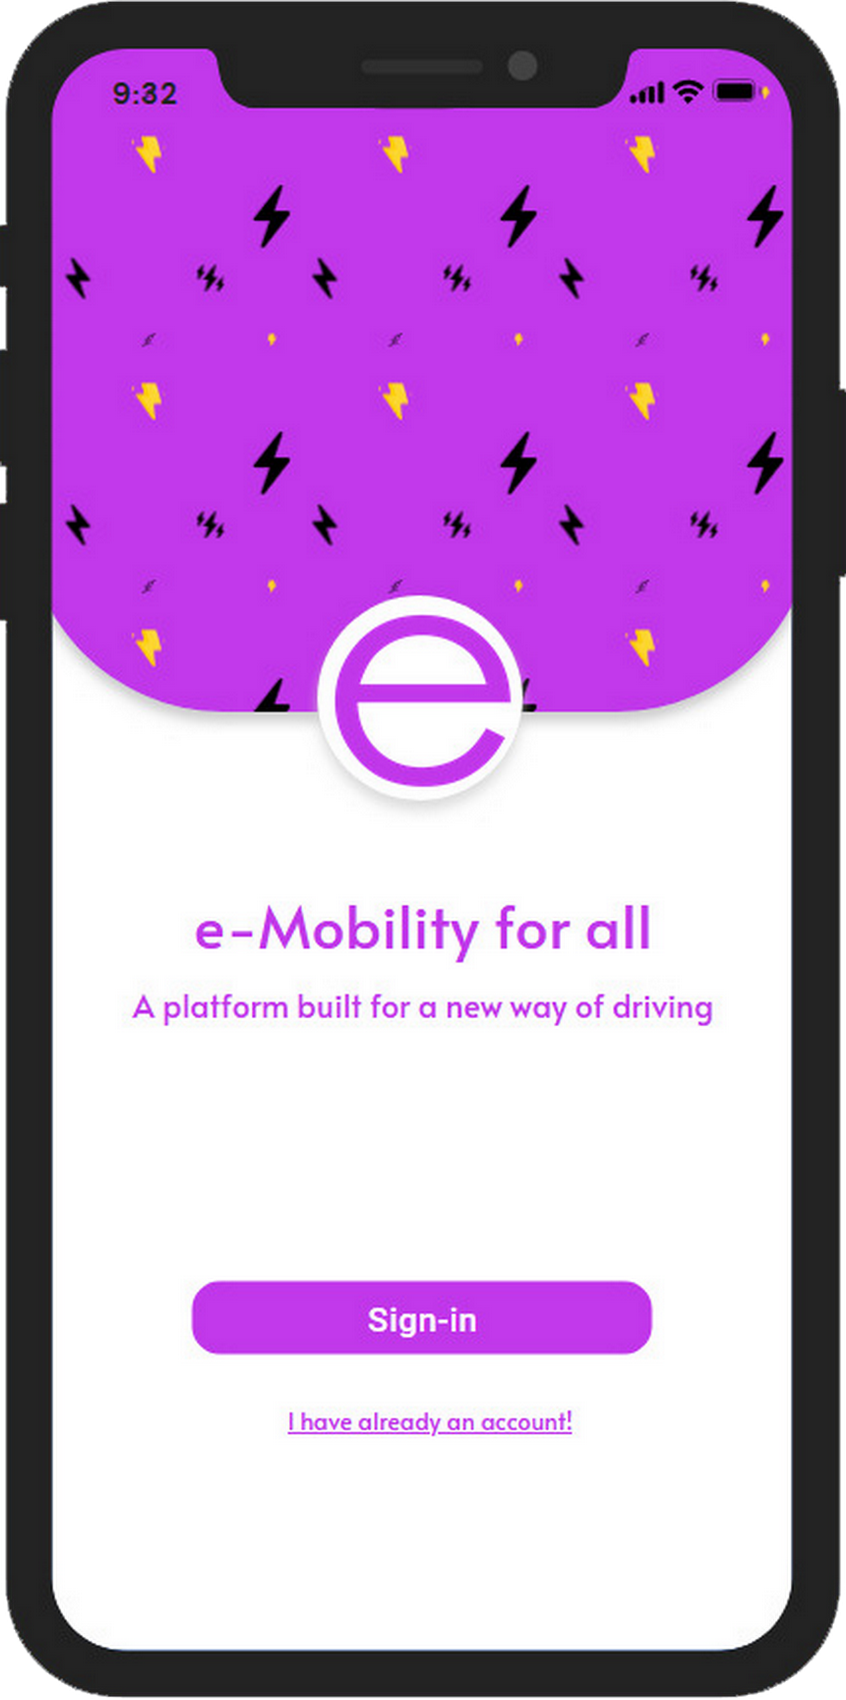
\includegraphics[width = 0.30\textwidth]{images/home.png}} &
\subfloat{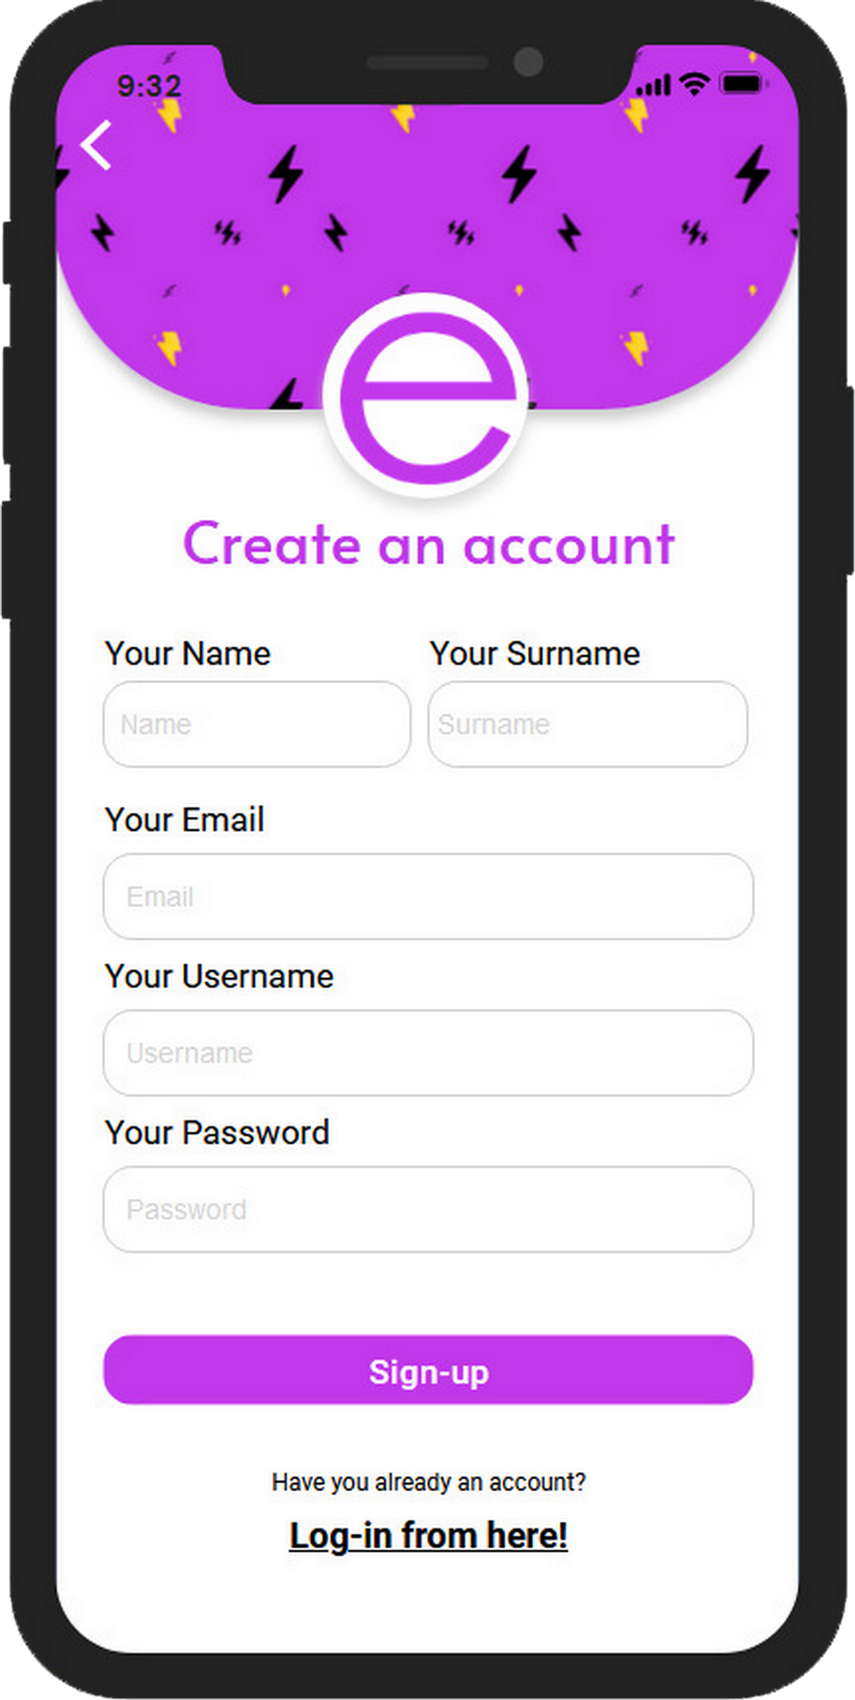
\includegraphics[width =0.30\textwidth]{images/signup.png}} &
\subfloat{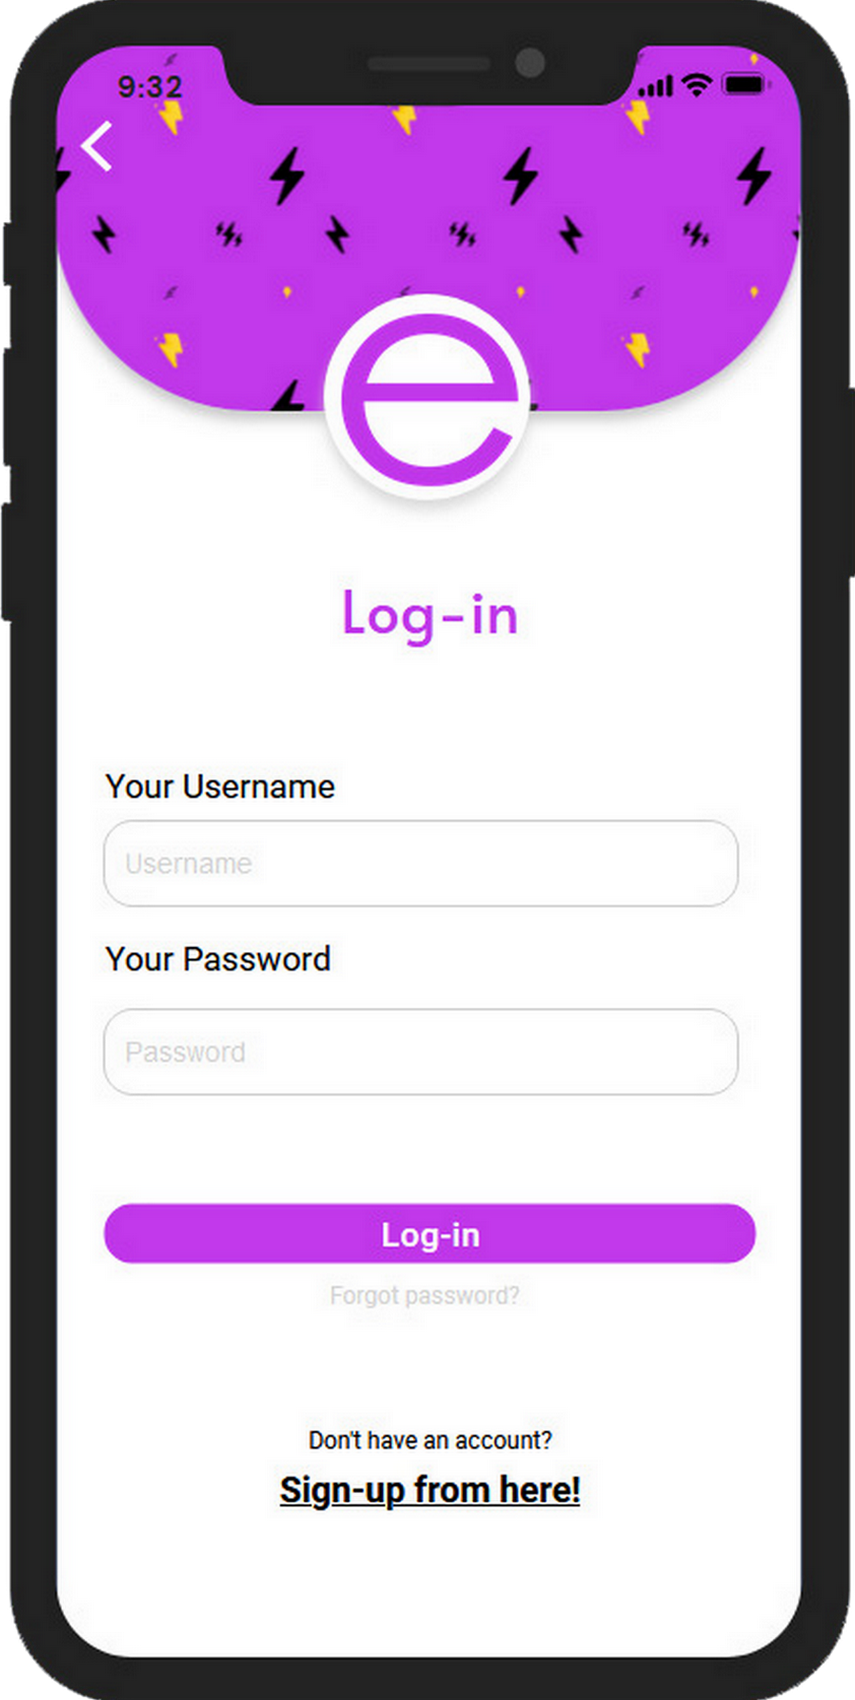
\includegraphics[width = 0.30\textwidth]{images/login.png}}
\end{tabular}
\end{figure}
%------------------
\begin{figure}[H]
\centering
\begin{tabular}{ccc}
\subfloat{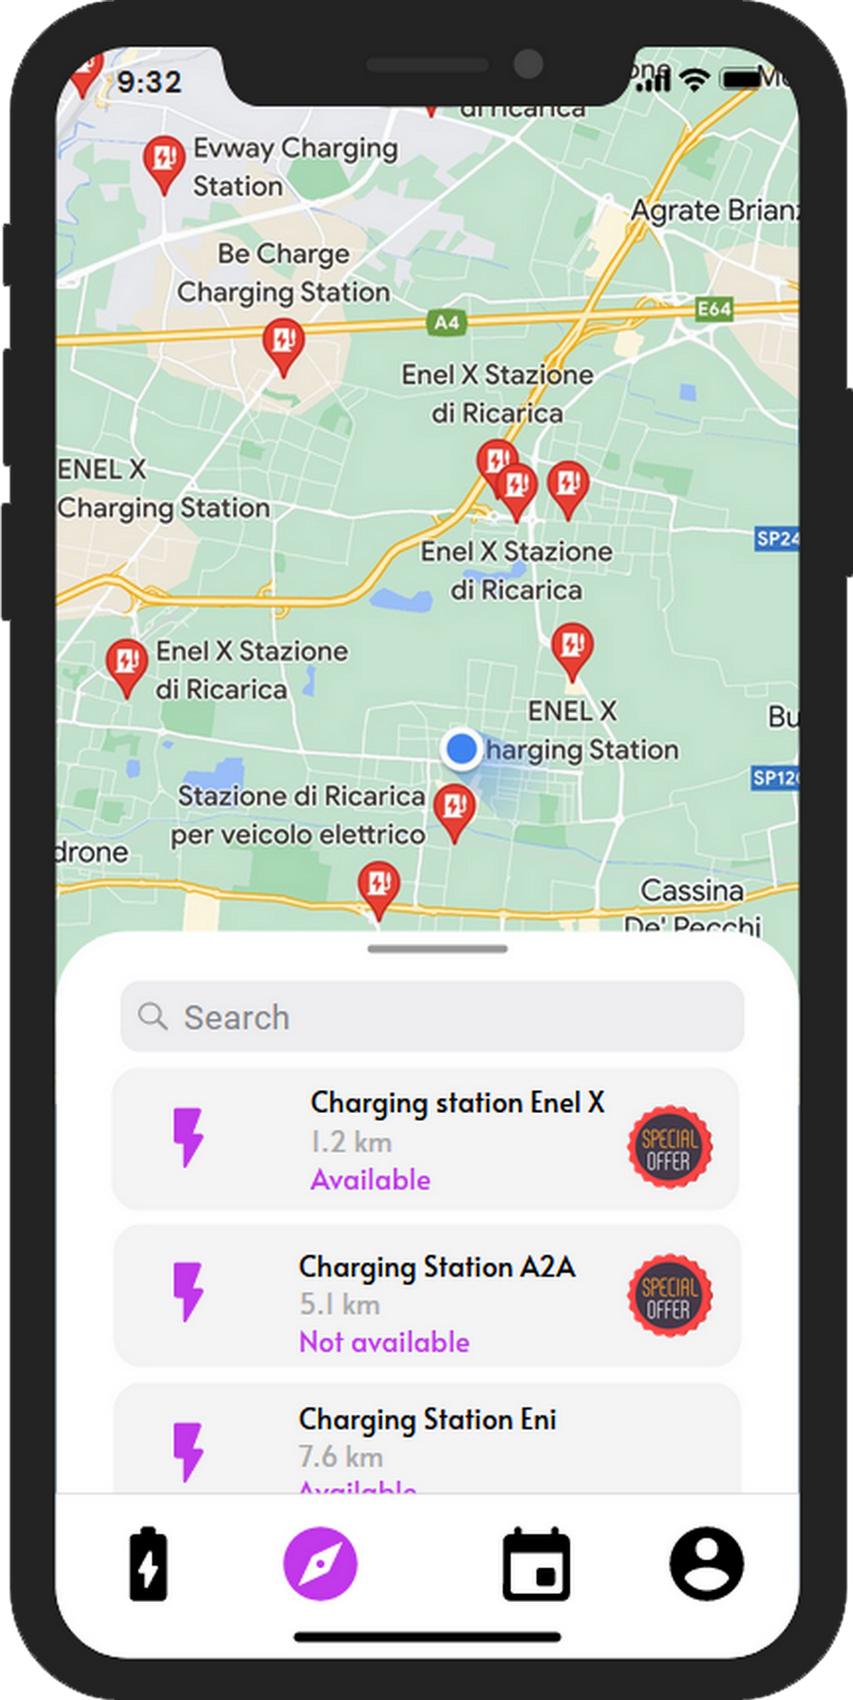
\includegraphics[width = 0.30\textwidth]{images/explore1.png}}&
\subfloat{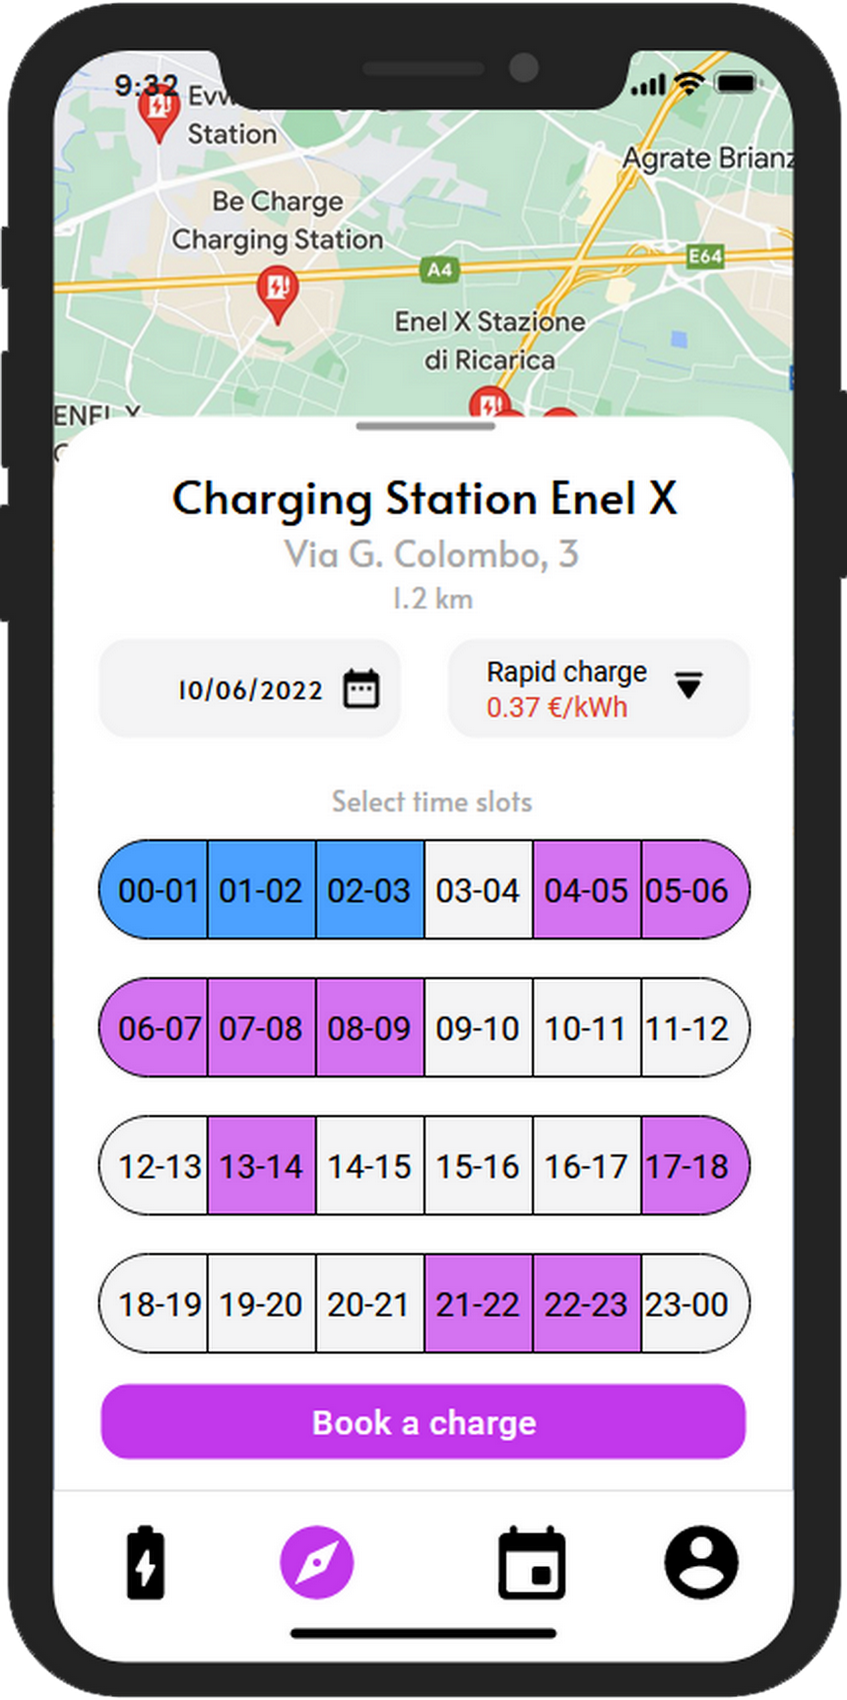
\includegraphics[width = 0.30\textwidth]{images/explore 2.png}}  &
\subfloat{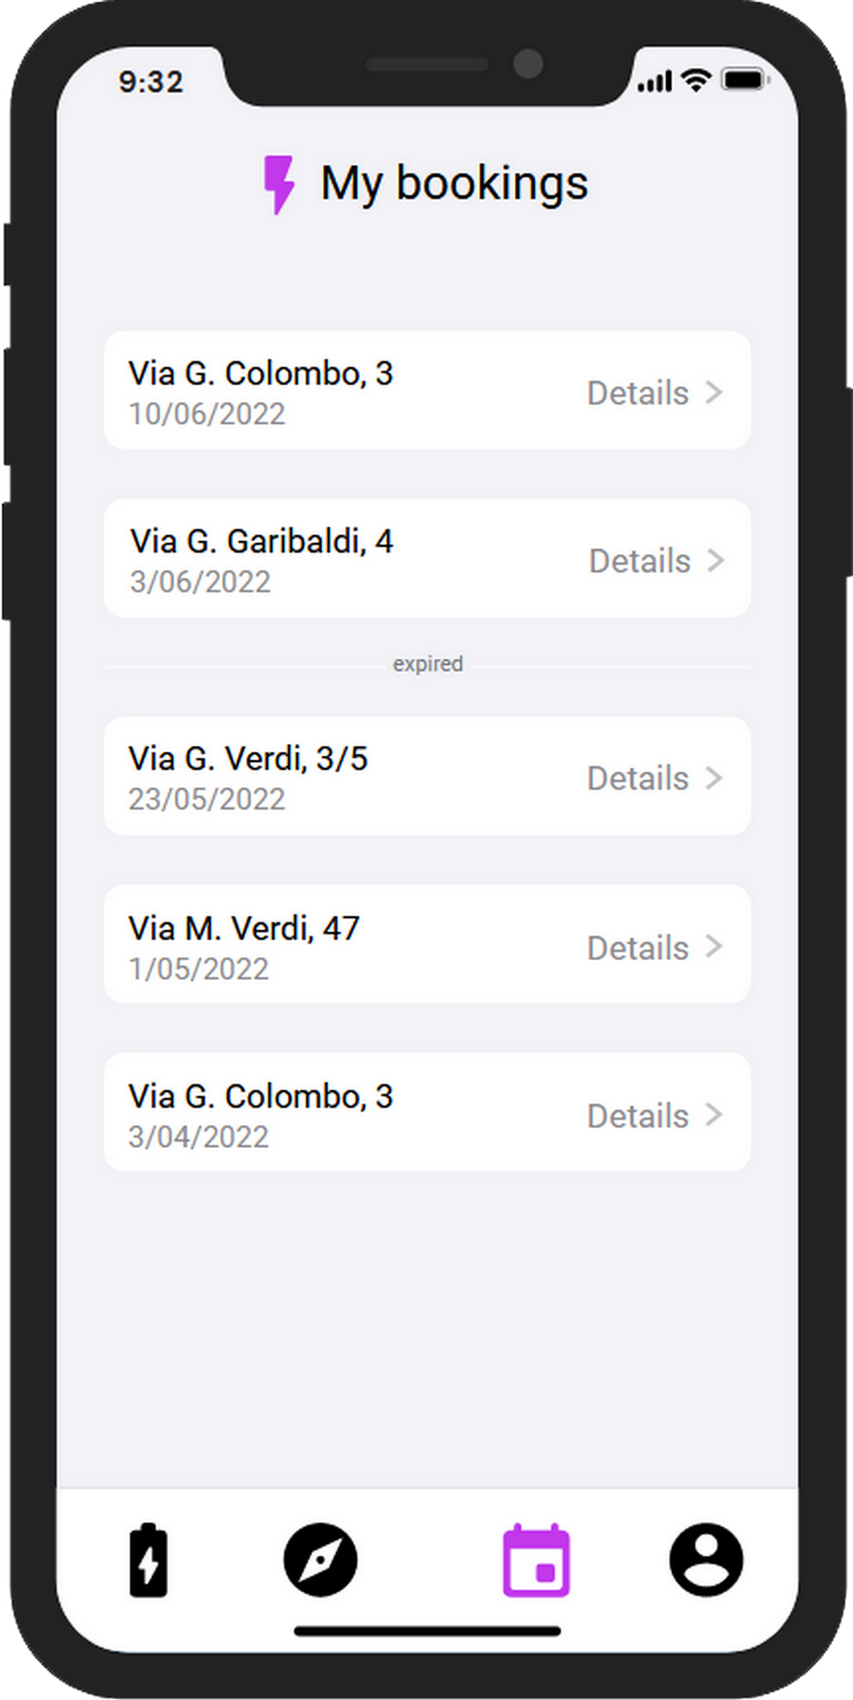
\includegraphics[width = 0.30\textwidth]{images/bookings.png}} \\
\subfloat{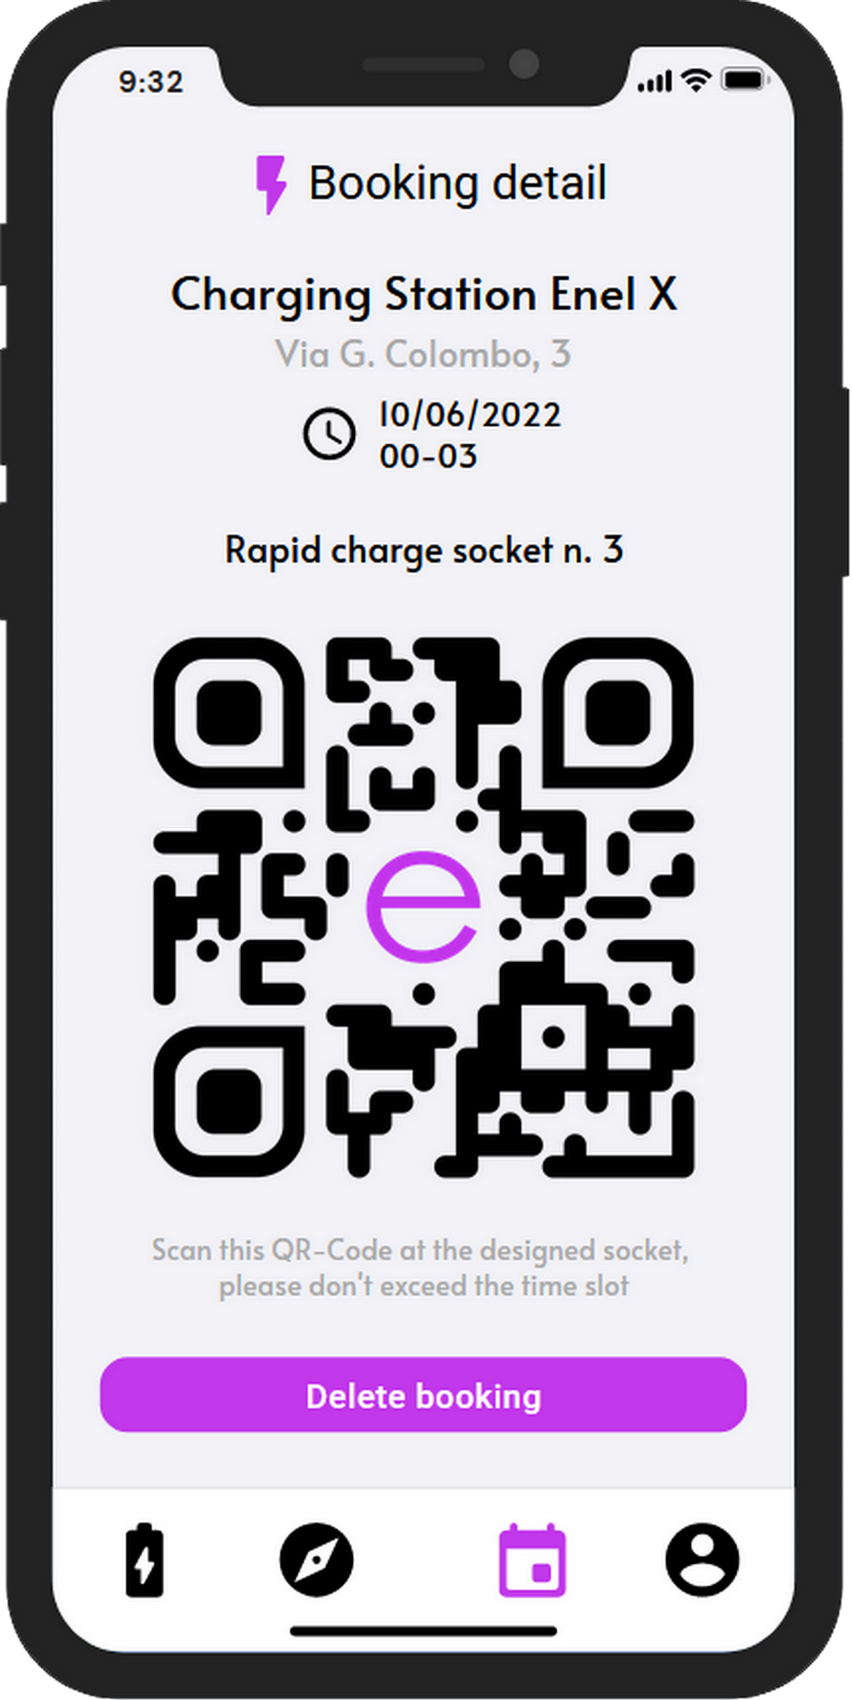
\includegraphics[width = 0.30\textwidth]{images/bookingdetail.png}} &
\subfloat{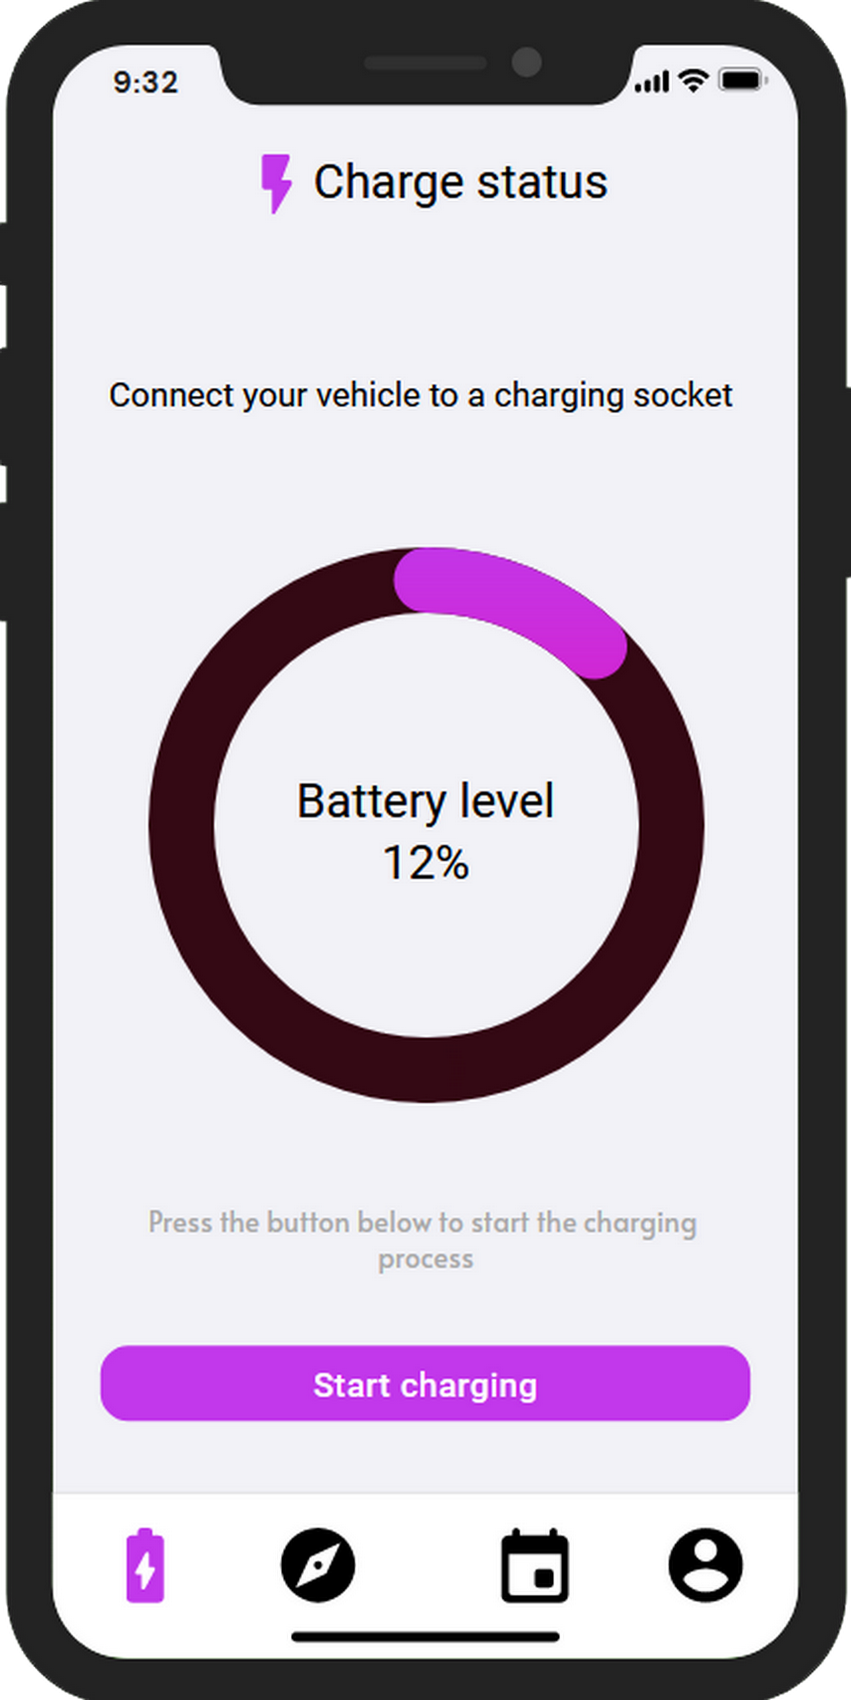
\includegraphics[width = 0.30\textwidth]{images/startcharge.png}}  &
\subfloat{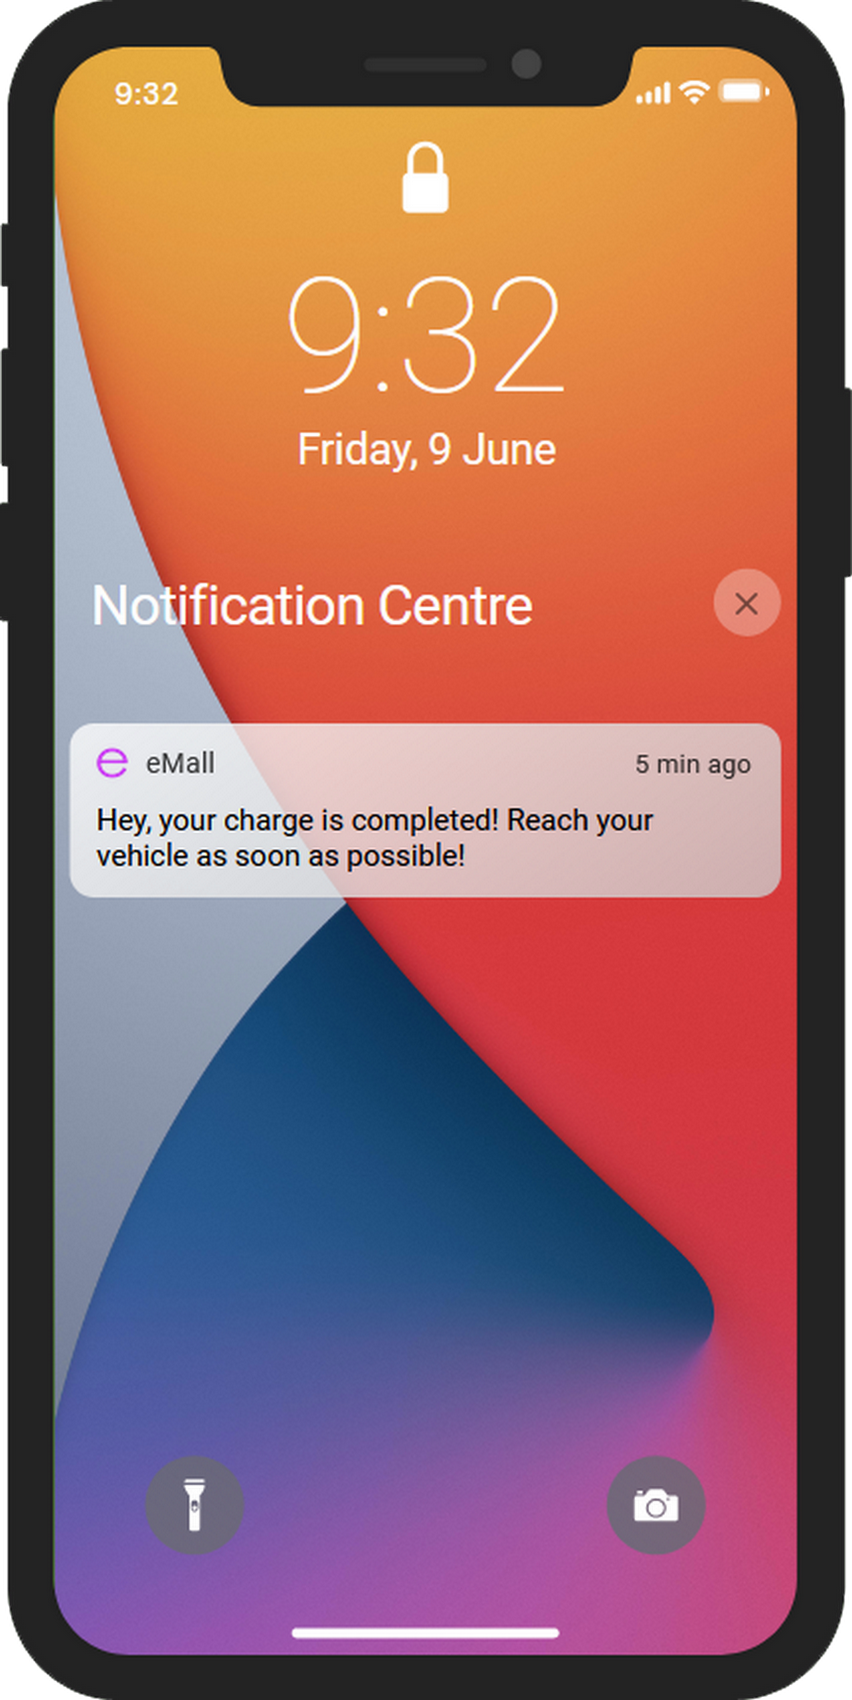
\includegraphics[width = 0.30\textwidth]{images/notific.png}}
\end{tabular}
\end{figure}
\begin{figure}[H]
\centering
\begin{tabular}{ccc}
\subfloat{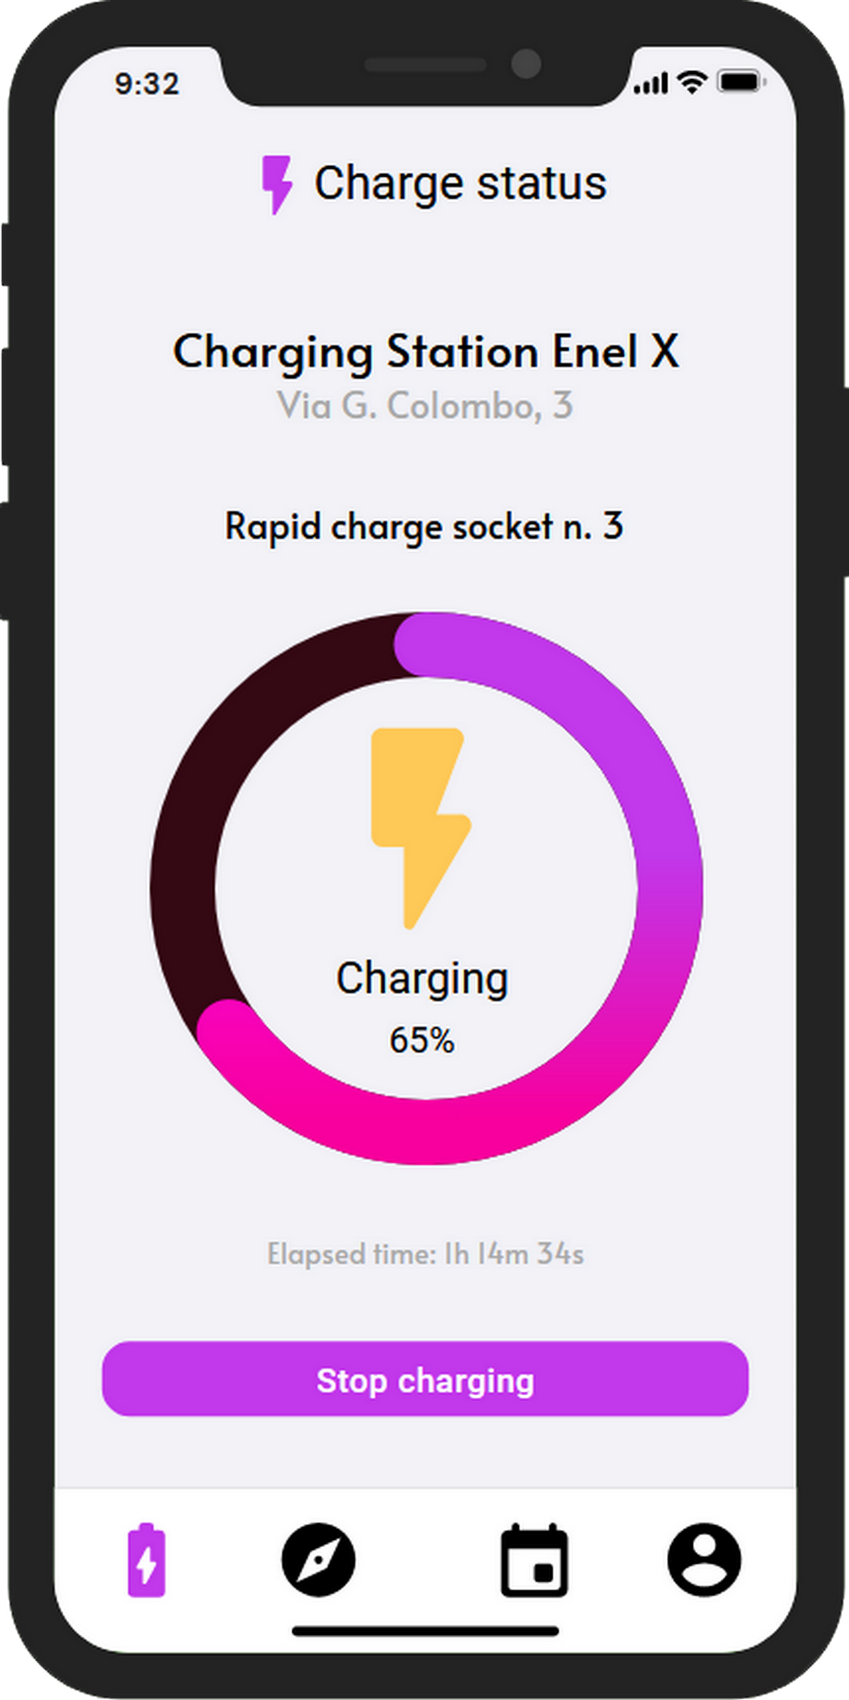
\includegraphics[width = 0.30\textwidth]{images/stopcharge.png}} &
\subfloat{
\includegraphics[width = 0.30\textwidth]{images/user.png}}
\end{tabular}
\end{figure}
\subsubsection{CPO interfaces}
\begin{figure}[H]
\centering
\begin{tabular}{ccc}
\subfloat{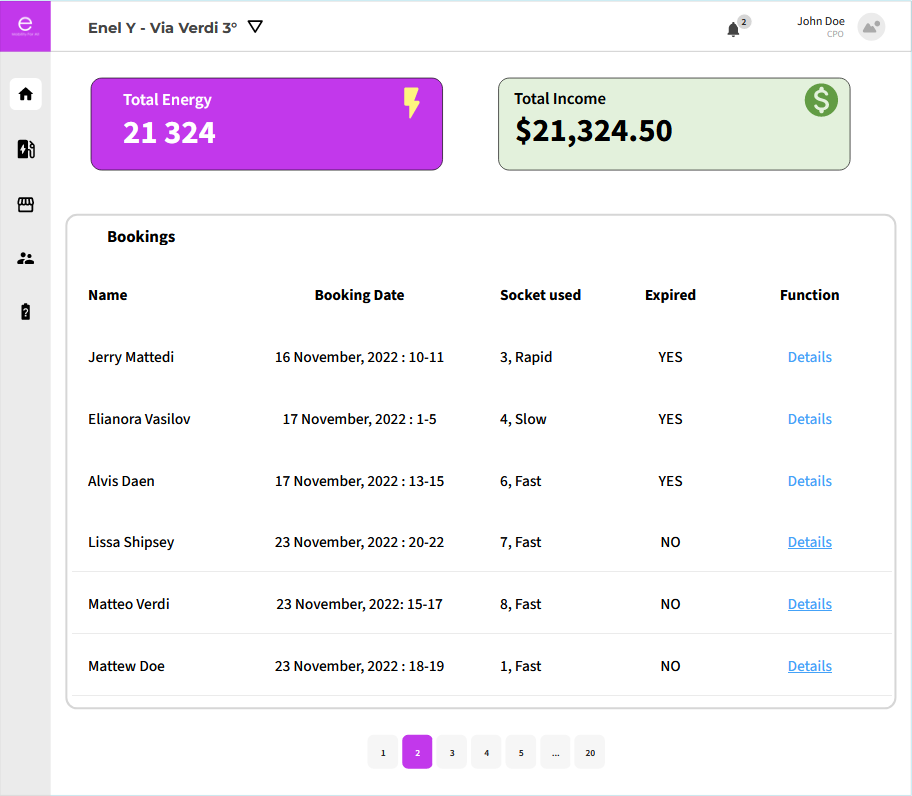
\includegraphics[width = 0.50\textwidth]{images/home2.png}} &
\subfloat{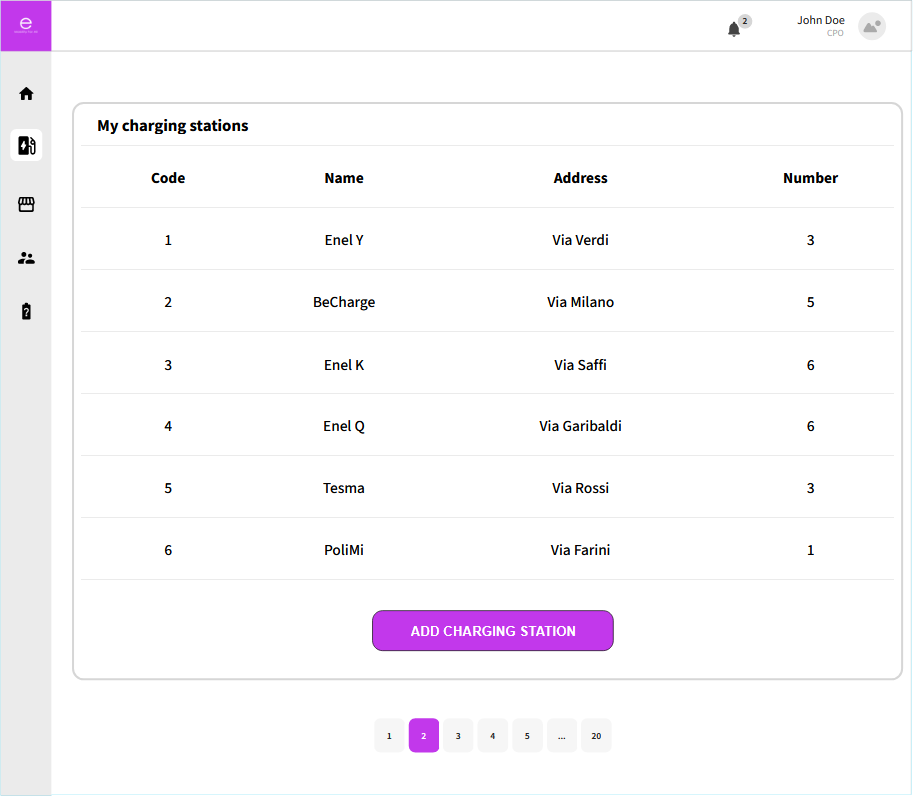
\includegraphics[width = 0.50\textwidth]{images/add.png}}\\
\subfloat{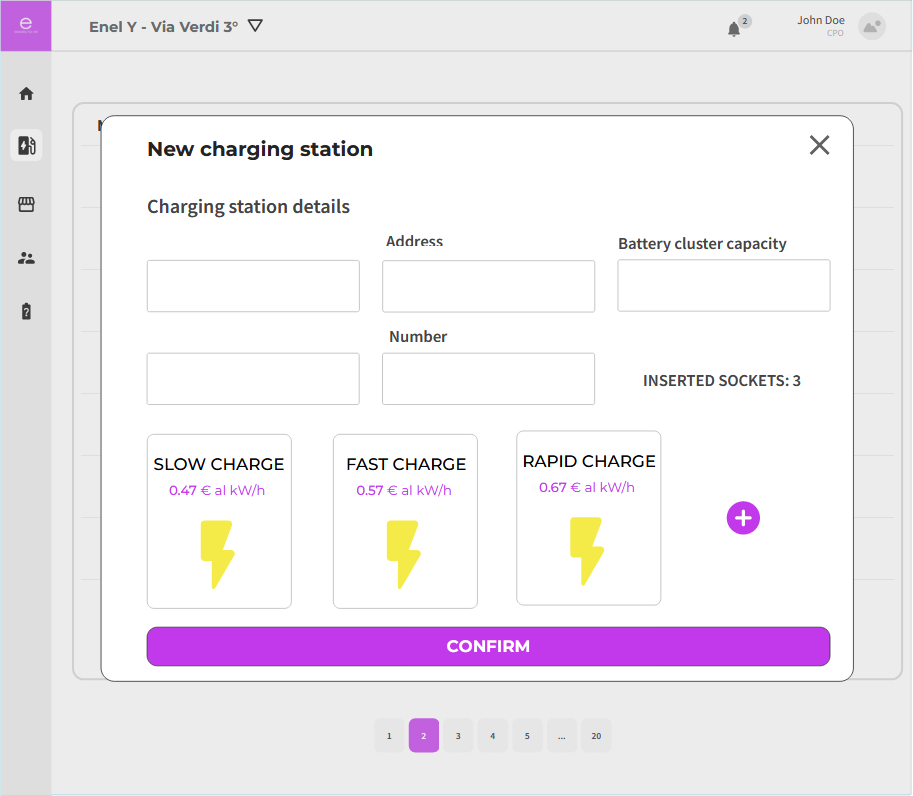
\includegraphics[width = 0.50\textwidth]{images/add2.png}} &
\subfloat{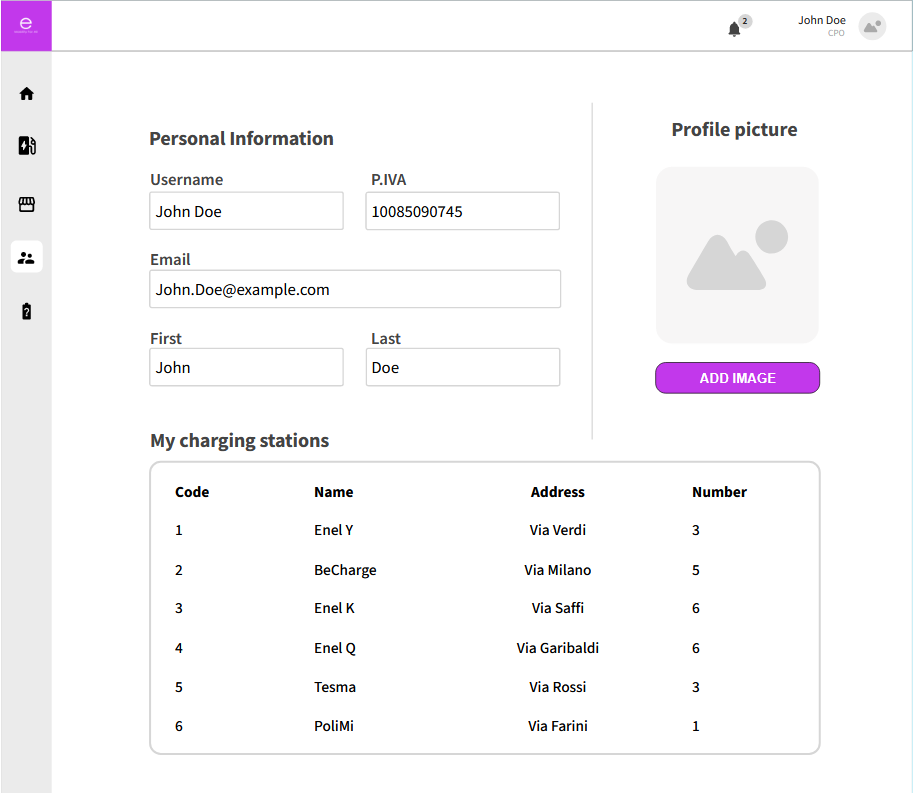
\includegraphics[width = 0.50\textwidth]{images/cpo.png}} \\
\subfloat{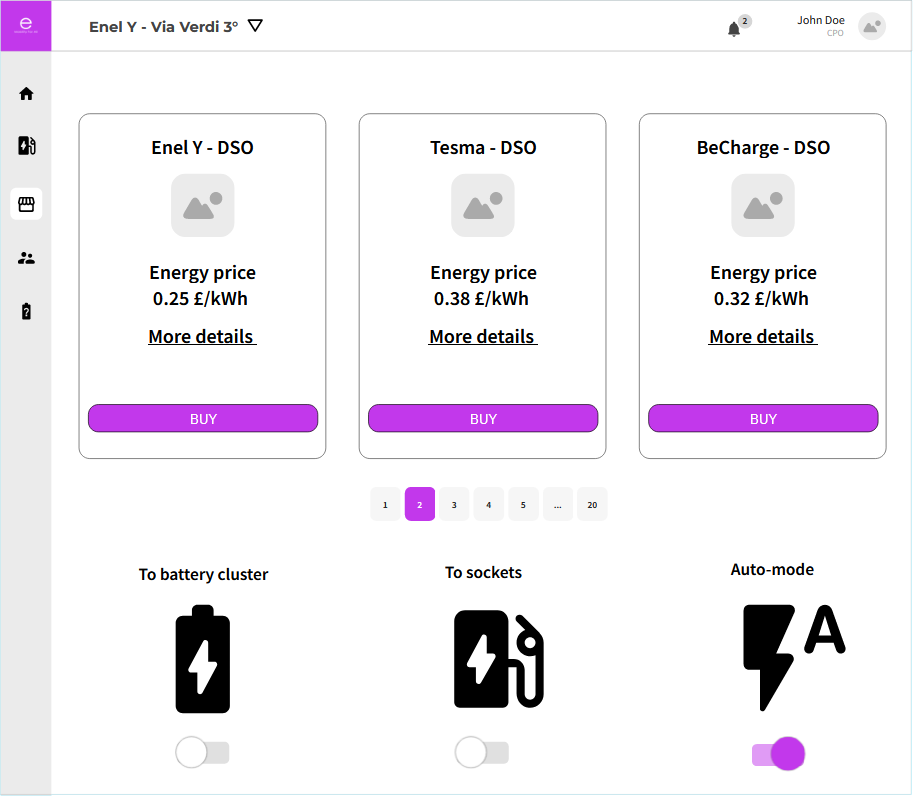
\includegraphics[width = 0.50\textwidth]{images/dso.png}} &
\subfloat{
\includegraphics[width = 0.50\textwidth]{images/battery.png}} \\
\end{tabular}
\end{figure}
\subsection{Hardware Interfaces}
This section describes the logical and physical characteristics of each interface between the software and the hardware components of the system.\\
In order to allow the entire system to function properly, some devices are required:
\begin {itemize}
    \item \textbf {smartphones} for end users equipped with GPS.
    \item \textbf {smartphones} or \textbf {PC} for CPOs to access their control panel via \textbf {web browser}.
    \item \textbf {QR-Code} scanner installed on the charging socket to allow end users' booking recognition.
\end {itemize}
\subsection{Software Interfaces}
This section describes the connections between the system and other specific software components.\\
The eMall system communicates with geolocation APIs to view the charging stations according to the criteria shown above, with bank APIs to substract automatically the amount of a charge. Moreover, the system should have an access to end user's vehicle APIs and end user's calendar APIs to proactively suggest a specific charging stations.
\subsection{Communication Interfaces}
This section describes the requirements associated with any communication function required by this system.\\
All the communications of the eMall infrastructure are made via the HTTP application layer protocol: obviously, all the devices using the platform must be connected via WiFi or mobile network (LTE/3G/4G/5G). Due to the fact that some of the interactions are real time, for example the communication between the charging sockets and the CPMS, is necessairly to use WebSocket protocol, which enables real time communication over HTTP.
\section{Functional Requirements}
\subsection{Use Cases Diagrams}
\begin{figure}[H]
    \centering
    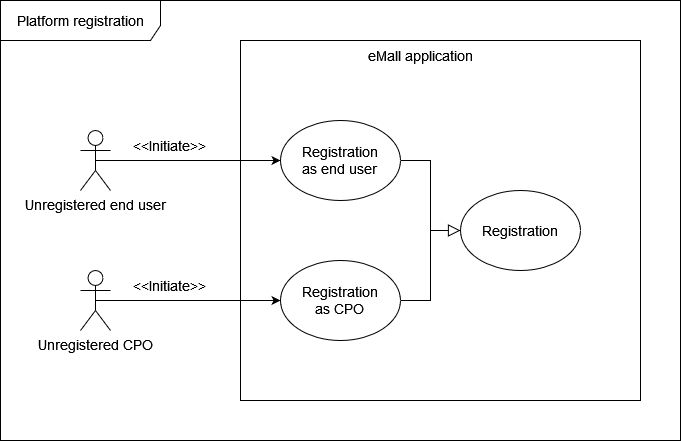
\includegraphics[width=\textwidth]{images/uc_registration.png}
    \caption{Registration operation use case diagram.}
    \label{fig:uc_registration}
\end{figure}
\begin{figure}[H]
    \centering
    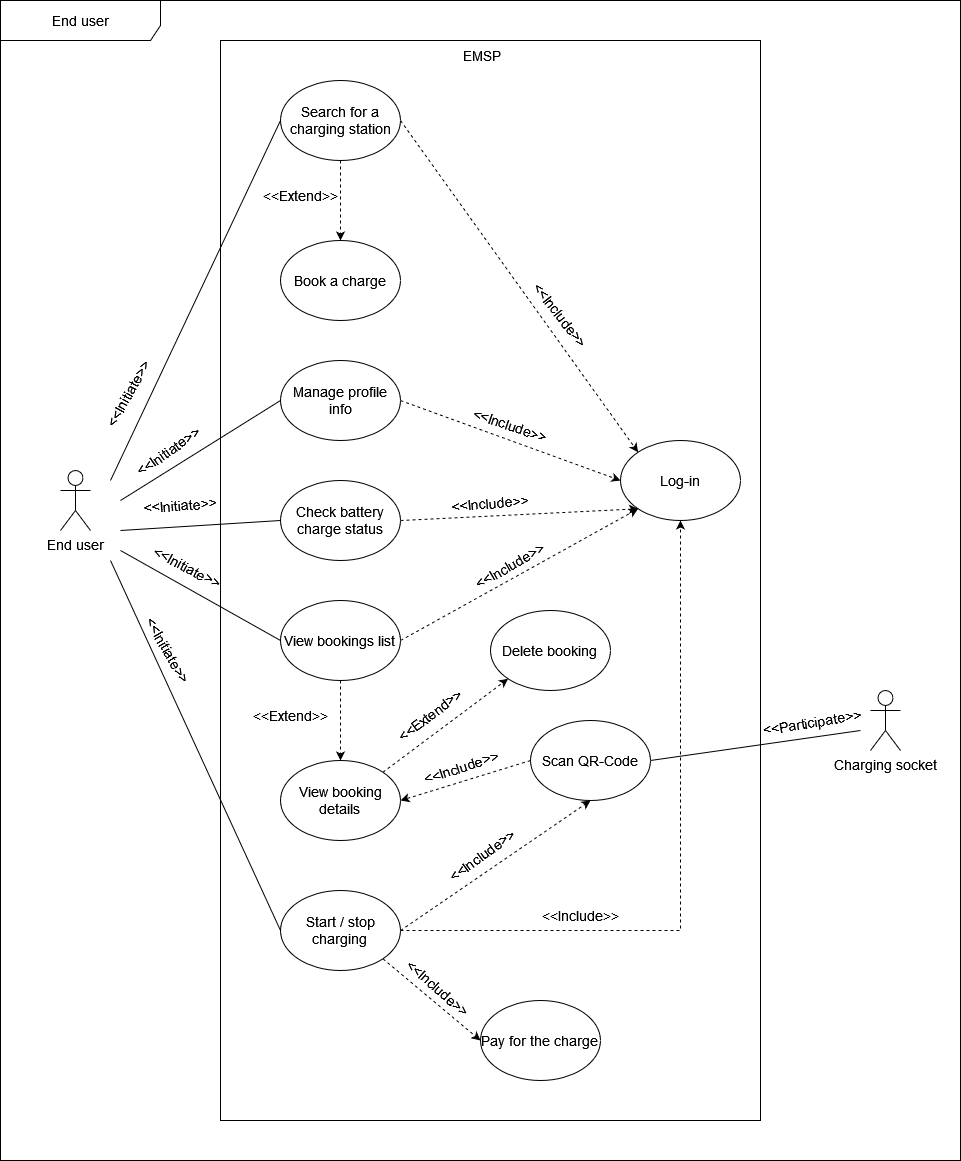
\includegraphics[width=\textwidth]{images/uc_user.png}
    \caption{End user's operations use case diagram.}
    \label{fig:uc_user}
\end{figure}
\begin{figure}[H]
    \centering
    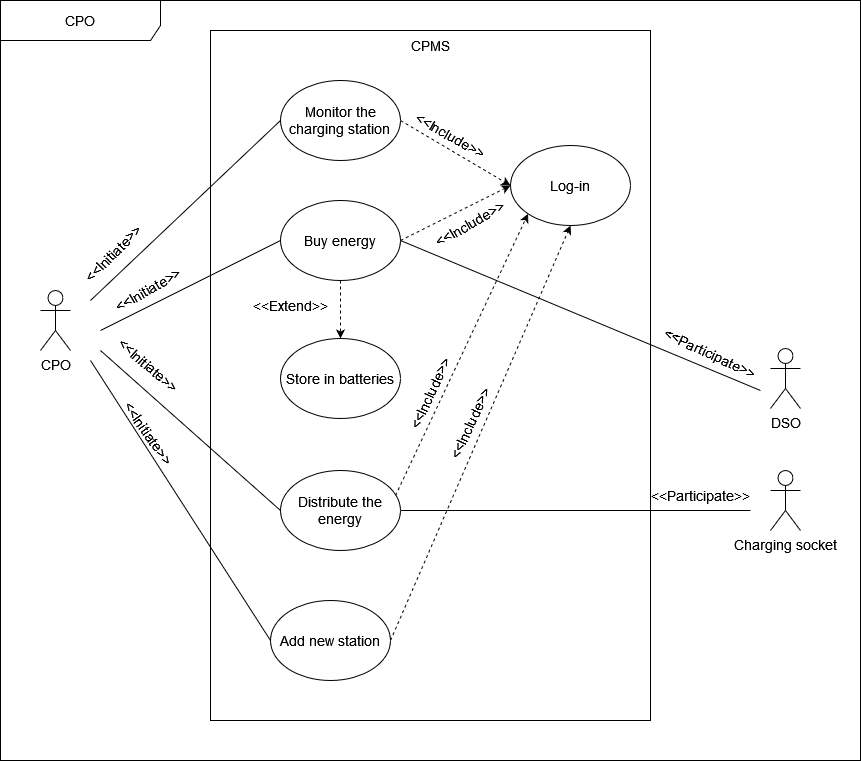
\includegraphics[width=\textwidth]{images/uc_CPO.png}
    \caption{CPO's operations use case diagram.}
    \label{fig:uc_cpo}
\end{figure}
\subsection{Use Cases Description}
\begin{table}[H]
\resizebox{\textwidth}{!}{%
\centering
\begin{tabular}{|
>{\columncolor[HTML]{B8C8D5}}c |l|}
\hline
Name            & Platform registration                     \\ \hline
ID              & UC.1                                      \\ \hline
Actors          & Unregistered End User, Unregistered CPO \\ \hline
Entry Condition & 1) The actor is running the application. \\ \hline
Event Flow &
  \begin{tabular}[c]{@{}l@{}} 
  1) The actor navigates to the sign-up page.\\ 
  2) The end user fills the sign-up form with name, surname, \\email, username and password.\\ 
  3) The unregistered CPO fills the sign-up form with name, surname, \\ email, username and password. The CPO also needs to insert \\some business data. \\
  4) The actor submits the registration.\\ 
  5) The system sends a confirmation email to verify the actor's email.\\
  6) The system stores the actor's data.\\ 
  7) The system redirects the actor to the log-in page.\end{tabular} \\ \hline
Exit Condition  & The actor signed-up correctly.         \\ \hline
Exceptions &
  \begin{tabular}[c]{@{}l@{}}
  1) The provided username or email are already registered.\\
  2) The actor doesn't fill the form with correct information.\\ \\ All \textit{execptions caused by user errors are notified by the}\\ \textit{system and managed in the Event Flow.}\end{tabular} \\ \hline
\end{tabular}
}
\end{table}
\begin{table}[H]
\resizebox{\textwidth}{!}{%
\centering
\begin{tabular}{|
>{\columncolor[HTML]{B8C8D5}}c |l|}
\hline
Name            & Platform log-in                           \\ \hline
ID              & UC.2                                      \\ \hline
Actors          & End User, CPO                           \\ \hline
Entry Condition & \begin{tabular}[c]{@{}l@{}} 1) The actor is running the application. \\ 
2) The actor is already registered.\end{tabular}\\ \hline
Event Flow &
  \begin{tabular}[c]{@{}l@{}}
  1) The actor navigates to the log-in page.\\ 
  2) The actor fills the log-in form with username and password.\\ 
  3) The actor submits the log-in.\\ 
  4) The system redirects the actor to the explore page.\end{tabular} \\ \hline
Exit Condition  & The actor is logged-in correctly.         \\ \hline
Exceptions &
  \begin{tabular}[c]{@{}l@{}}
  1) The provided username is incorrect. \\2) The provided password is incorrect.\\ \\ \textit{execptions caused by user errors are notified by the}\\ \textit{system and managed in the Event Flow.}\end{tabular} \\ \hline
\end{tabular}
}
\end{table}

\begin{table}[H]
\resizebox{\textwidth}{!}{%
\centering
\begin{tabular}{|
>{\columncolor[HTML]{B8C8D5}}c |l|}
\hline
Name            & Book a charge                                                                                                                                \\ \hline
ID              & UC.3                                                                                                                                         \\ \hline
Actors          & End User                                                                                                                                    \\ \hline
Entry Condition & \begin{tabular}[c]{@{}l@{}}1) The end user is running the application.\\ 2) The end user is logged-in. \\3) The end user is in the explore page.\end{tabular}                        \\ \hline
Event Flow &
  \begin{tabular}[c]{@{}l@{}}1) The end user is looking for a charging station to charge\\his vehicle according to system's suggestions.\\
  2) The end user selects the desired charging station.\\
  3) The end user selects the date and the charging socket type of\\    the charging station.\\
  4) The end user selects the desired time slot, if it's free.\\ 
  5) The end user presses the booking button.\end{tabular} \\ \hline
Exit Condition  & \begin{tabular}[c]{@{}l@{}}
The end user has successfully booked the charge for his vehicle\\    at the desired charging station to an assigned charging socket in\\ the designed time slot.\end{tabular} \\ \hline
Exceptions &
  \begin{tabular}[c]{@{}l@{}}
 1) The user on the booking page waits too long in selecting \\the desired time slot, this way another user books the desired\\ time slot faster than the other. The first user does not see this \\change and therefore selects that time slot, so the system tells\\ him through a notification that there has been an error and that\\ he must restart from point 2 of the event flows. \end{tabular} \\ \hline
\end{tabular}
}
\end{table}

\begin{table}[H]
\resizebox{\textwidth}{!}{%
\centering
\begin{tabular}{|
>{\columncolor[HTML]{B8C8D5}}c |l|}
\hline
Name            & Manage booking                                                                                                         \\ \hline
ID              & UC.4                                                                                                                  \\ \hline
Actors          & End User                                                                                                             \\ \hline
Entry Condition & \begin{tabular}[c]{@{}l@{}}
1) The end user is running the application.\\
2) The end user is logged-in.\\
3) The end user has already booked a charge.\\
4) The end user is in the bookings view page.\end{tabular} \\ \hline
Event Flow &
  \begin{tabular}[c]{@{}l@{}}
  1) The end user views his current bookings.\\ 
  2) The end user views his expired bookings. \\
  3) The end user selects a booking.\\ 
  4) The end user views all the details about the selected booking.\\ 
  5) The end user views the QR-Code of the booking.\end{tabular} \\ \hline
Exit Condition  &The user has viewed the booking.                                                                         \\ \hline
Exceptions      &\textit{None}                                                                                                                \\ \hline
\end{tabular}
}
\end{table}

\begin{table}[H]
\resizebox{\textwidth}{!}{%
\centering
\begin{tabular}{|
>{\columncolor[HTML]{B8C8D5}}c |l|}
\hline
Name           & Delete Booking                                \\ \hline
ID             & UC.5                                          \\ \hline
Actors         & End User                                     \\ \hline
Entry Condition &
  \begin{tabular}[c]{@{}l@{}}
  1) The end user is running the application.\\
2) The end user is logged-in.\\
3) The end user has already booked a charge.\\
4) The end user is in the bookings view page.\end{tabular} \\ \hline
Event Flow &
  \begin{tabular}[c]{@{}l@{}}
  1) The end user selects the booking to delete.\\
  2) The end user deletes the booking by pressing the appropriate\\   button.\end{tabular} \\ \hline
Exit Condition & The end user has deleted successfully the booking. \\ \hline
Exceptions     & \textit{None}                                        \\ \hline
\end{tabular}
}
\end{table}

\begin{table}[H]
\resizebox{\textwidth}{!}{%
\centering
\begin{tabular}{|
>{\columncolor[HTML]{B8C8D5}}c |l|}
\hline
Name            & Charging process                                                                                         \\ \hline
ID              & UC.6                                                                                                                     \\ \hline
Actors          & End User, Charging Socket                                                                                                \\ \hline
Entry Condition & \begin{tabular}[c]{@{}l@{}}
1) The end user is running the application.\\
2) The end user is logged-in.\\
3) The end user has already booked a charge.\\ 
4) The end user has a QR-Code.\\
5) The charging socket is installed.\end{tabular} \\ \hline
Event Flow &
  \begin{tabular}[c]{@{}l@{}}
  1) The end user goes to the assigned charging socket.\\
  2) The end user scans the Qr-Code of the booking \\using the QR-Code scanner on the charging socket.\\ 
  3) The system validates the booking.\\
  4) The end user charges his vehicle.\\
  4) The system notifies the user that the charge is completed.\\
  5) The system subtracts automatically the price of the charge.\end{tabular} \\ \hline
Exit Condition  &
The system allows the charging request and substratcs the related money.                                                  \\ \hline
Exceptions      & \begin{tabular}[c]{@{}l@{}}1) The Qr-Code is invalid or expired, in this case the charging process\\   doesn't start.\\
2) If the end user does not have enough money on his payment method, \\ the system tries, periodically, to subtract the amount of charge.\end{tabular}  \\ \hline
\end{tabular}
}
\end{table}

\begin{table}[H]
\resizebox{\textwidth}{!}{%
\centering
\begin{tabular}{|
>{\columncolor[HTML]{B8C8D5}}c |l|}
\hline
Name           & Purchase of energy                   \\ \hline
ID             & UC.7                                \\ \hline
Actors         & CPO, DSO                            \\ \hline
Entry Condition &
  \begin{tabular}[c]{@{}l@{}}
  1) The CPO is running the application.\\
  2) The CPO is logged-in.\\
  3) The CPO owns the charging station.\\
  4) The DSO has an offer for the energy.\end{tabular} \\ \hline
Event Flow &
  \begin{tabular}[c]{@{}l@{}}
  1) The CPO decides to buy energy for his charging station.\\ 
  2) The CPO makes a purchase of energy from a DSO through \\the CPMS.\\ 
  3) The CPO can decide whether to store the purchased energy. \\4) The CPO can decide whether to distribute the purchased \\
  energy to charging sockets.    \end{tabular} \\ \hline
Exit Condition & The CPO has bought energy from the DSO. \\ \hline
Exceptions     & None                              \\ \hline
\end{tabular}
}
\end{table}

\begin{table}[H]
\resizebox{\textwidth}{!}{%
\centering
\begin{tabular}{|
>{\columncolor[HTML]{B8C8D5}}c |l|}
\hline
Name           & Manage charging station            \\ \hline
ID             & UC.8                               \\ \hline
Actors         & CPO              \\ \hline
Entry Condition &
  \begin{tabular}[c]{@{}l@{}}
  1) The CPO is running the application.\\ 
    2) The CPO is logged-in.\\
  3) The CPO owns the charging station.\\
  \end{tabular} \\ \hline
Event Flow &
  \begin{tabular}[c]{@{}l@{}}
  1) The CPO visualizes the internal status of the station.\\
  2) The CPO visualizes the external status of the station.\\ 
  \end{tabular} \\ \hline
Exit Condition & The CPO has managed the status of his charging station. \\ \hline
Exceptions     & None                             \\ \hline
\end{tabular}
}
\end{table}

\begin{table}[H]
\resizebox{\textwidth}{!}{%
\centering
\begin{tabular}{|
>{\columncolor[HTML]{B8C8D5}}c |l|}
\hline
Name            & Add a charging station                                                                                                           \\ \hline
ID              & UC.9                                                                                                                             \\ \hline
Actors          & CPO                                                                                                                              \\ \hline
Entry Condition & \begin{tabular}[c]{@{}l@{}}
1) The CPO is running the application.\\ 
 2) The CPO is logged-in.\\
3) The CPO is in the add charging station page.\end{tabular} \\ \hline
Event Flow &
  \begin{tabular}[c]{@{}l@{}}
  1) The CPO decides to register a new charging station.\\ 
  2) The CPO fills the form with the infrastructure data of the charging\\ station.\\ 
  3) The system stores the new charging station's data.\end{tabular} \\ \hline
Exit Condition  & A new charging station has been created by the CPO.                                                                                 \\ \hline
Exceptions      & \begin{tabular}[c]{@{}l@{}}1) If the CPO fills the form with incorrect data, the system notifies \\ him the error.\\ 2) If the infrastructure data are already registered, the system \\doesn't store the data and notifies this error to the user.\end{tabular}   \\ \hline
\end{tabular}
}
\end{table}
\subsection{Sequence Diagrams}
\begin{figure}[H]
    \centering
    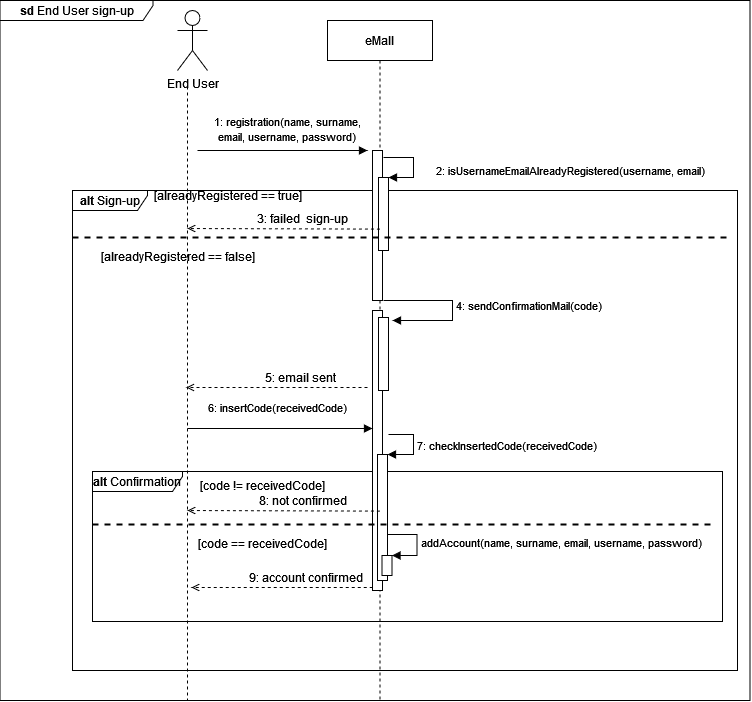
\includegraphics[width=\textwidth]{images/sd_registration_enduser.png}
    \caption{End user's registration sequence diagram.}
    \label{fig:sd_end_user}
\end{figure}
\begin{figure}[H]
    \centering
    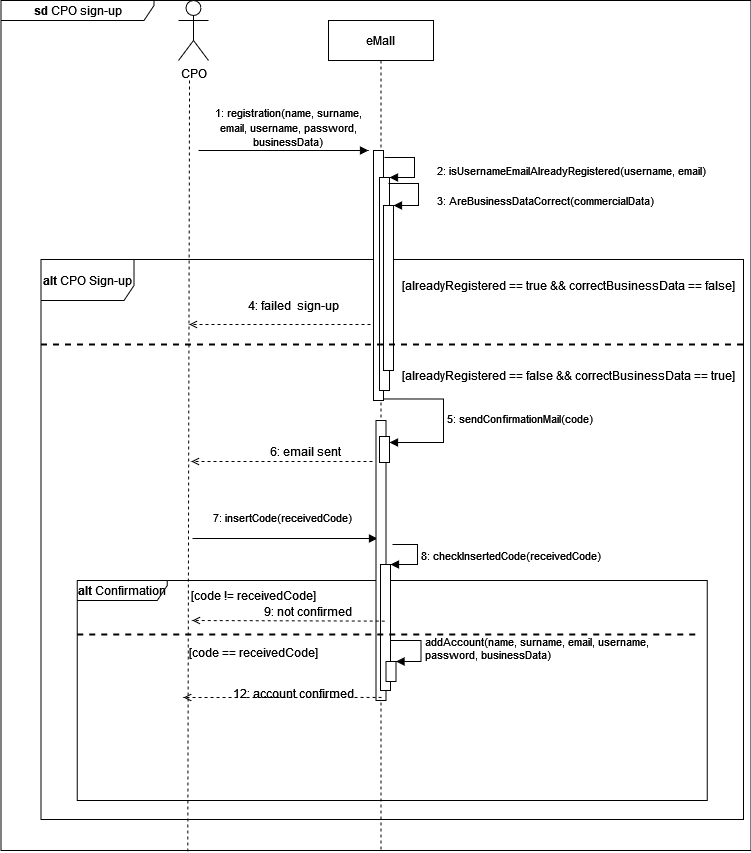
\includegraphics[width=\textwidth]{images/sd_registration_cpo.png}
    \caption{CPO's registration sequence diagram.}
    \label{fig:sd_cpo}
\end{figure}
\begin{figure}[H]
    \centering
    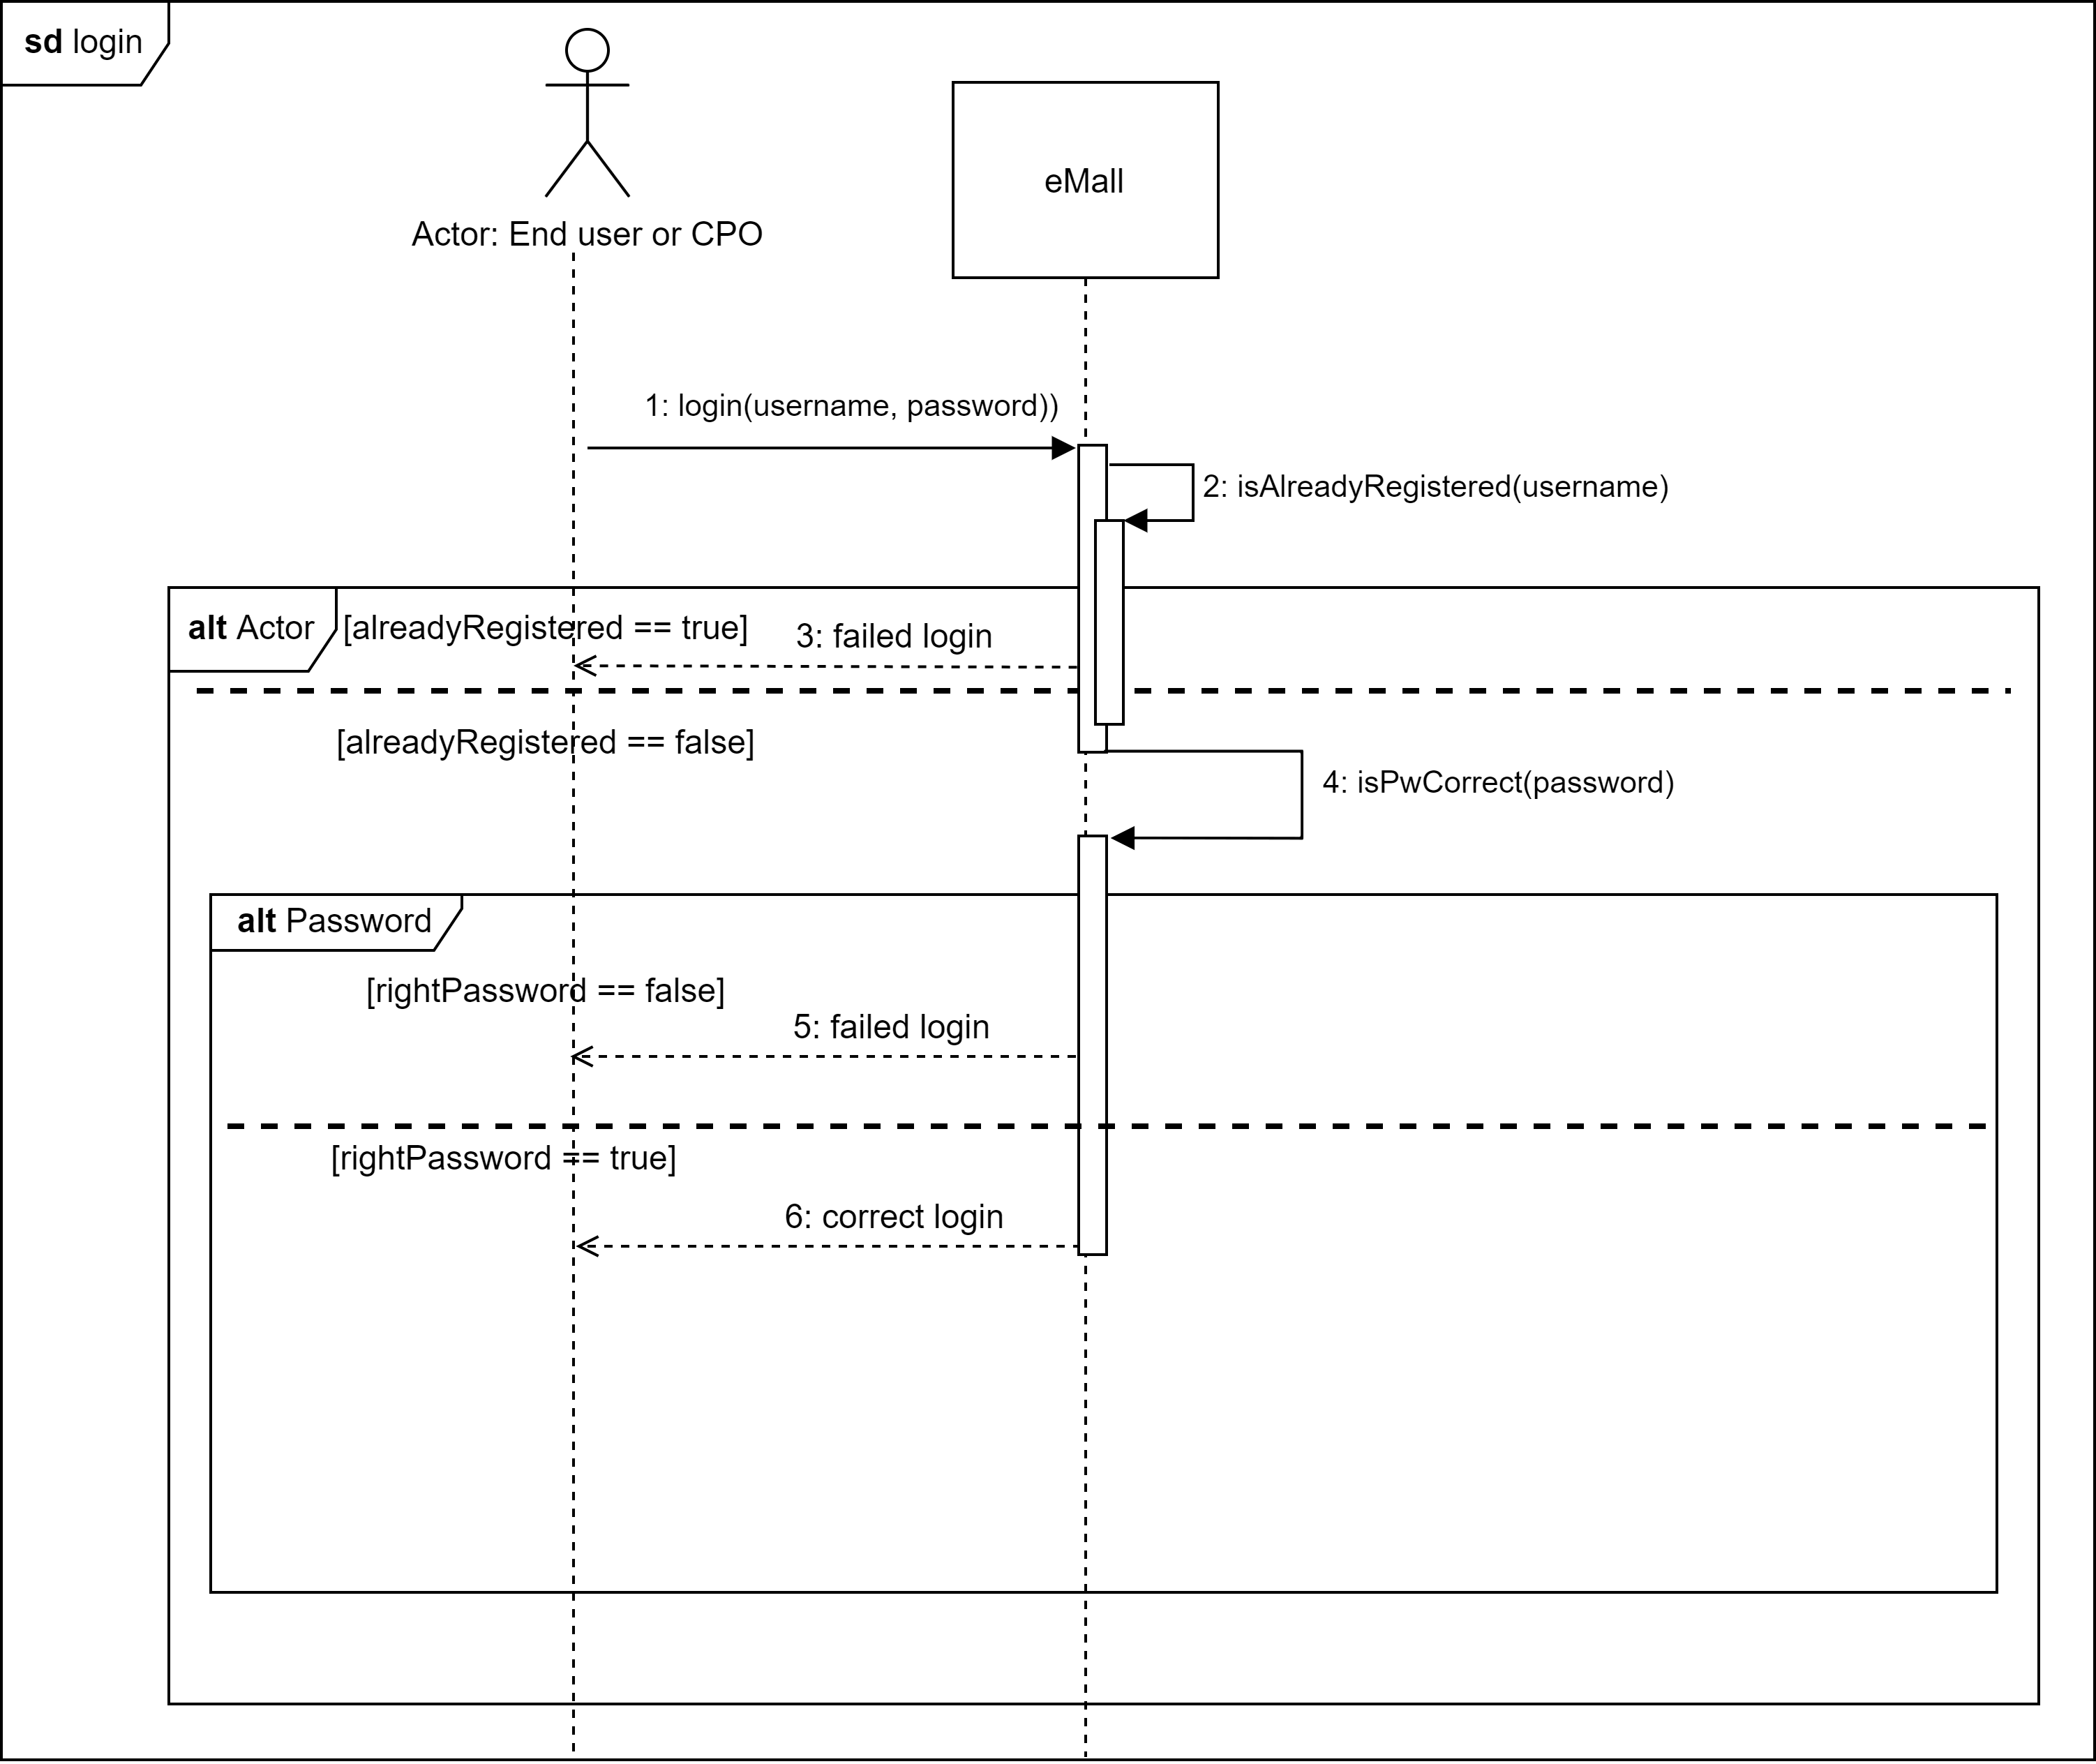
\includegraphics[width=\textwidth]{images/sd_login.png}
    \caption{Login sequence diagram.}
    \label{fig:sd_login}
\end{figure}
\begin{figure}[H]
    \centering
    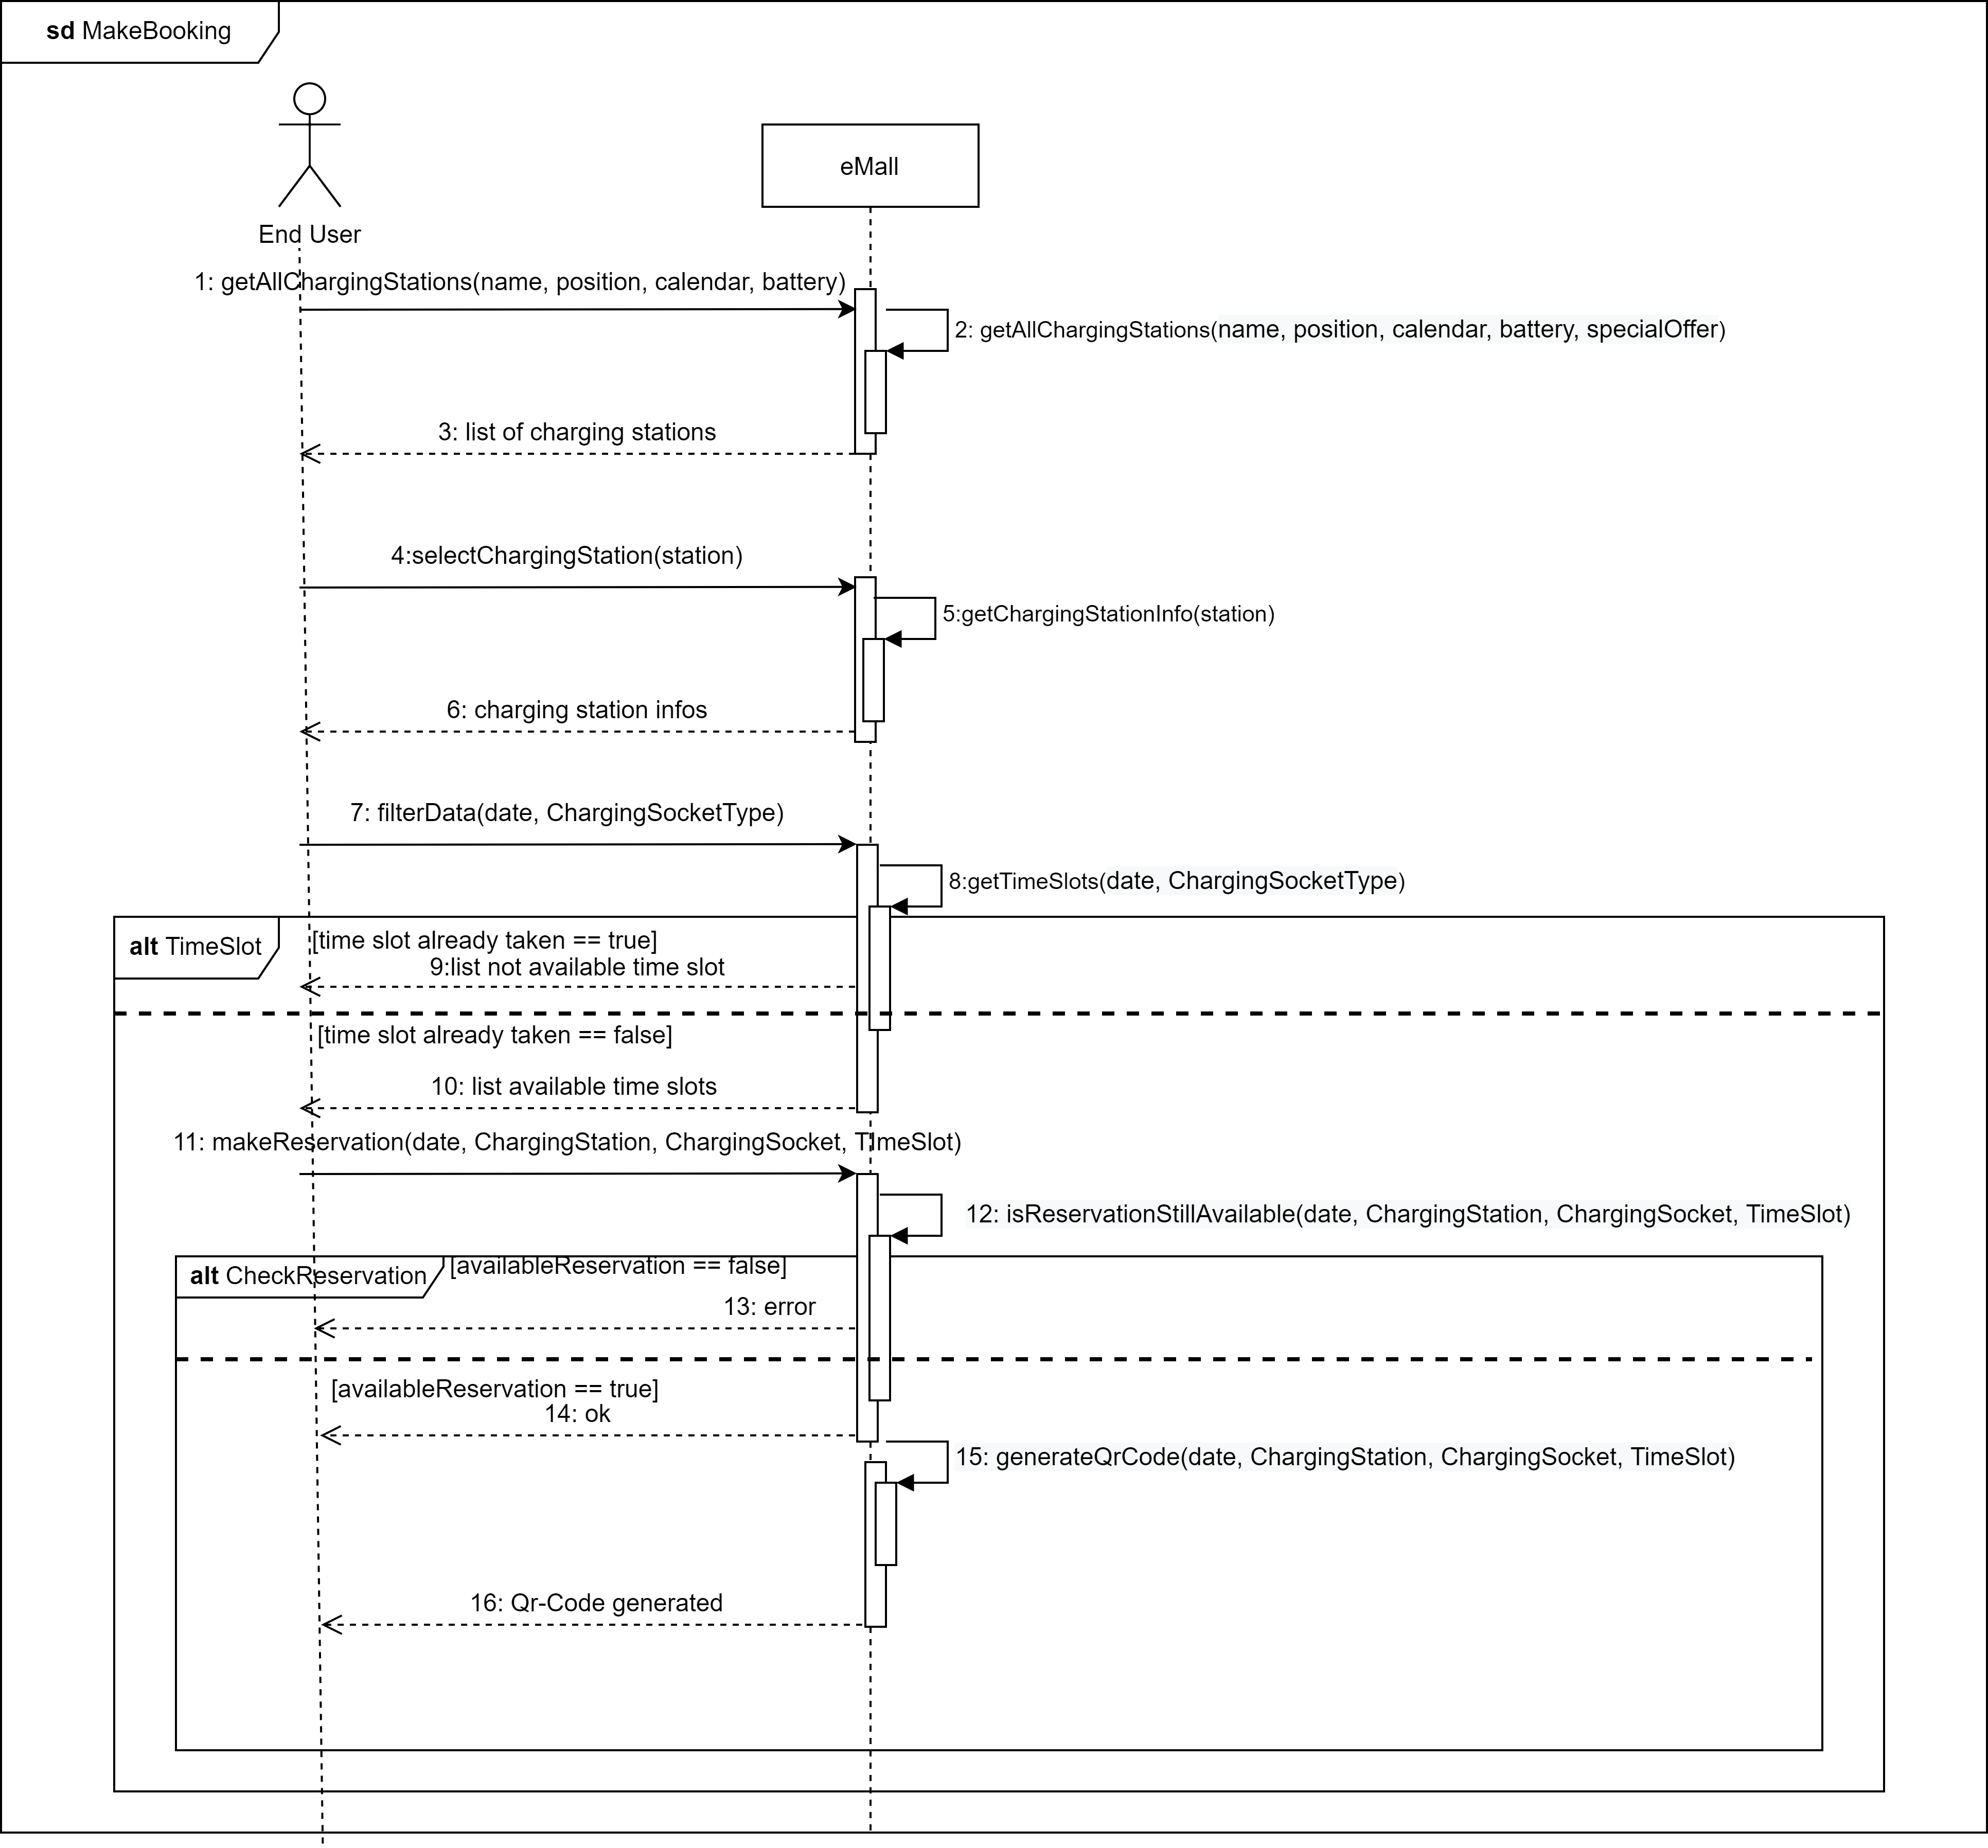
\includegraphics[width=\textwidth]{images/sd_makeBooking.png}
    \caption{End user booking a charge sequence diagram.}
    \label{fig:sd_booking_charge}
\end{figure}
\begin{figure}[H]
    \centering
    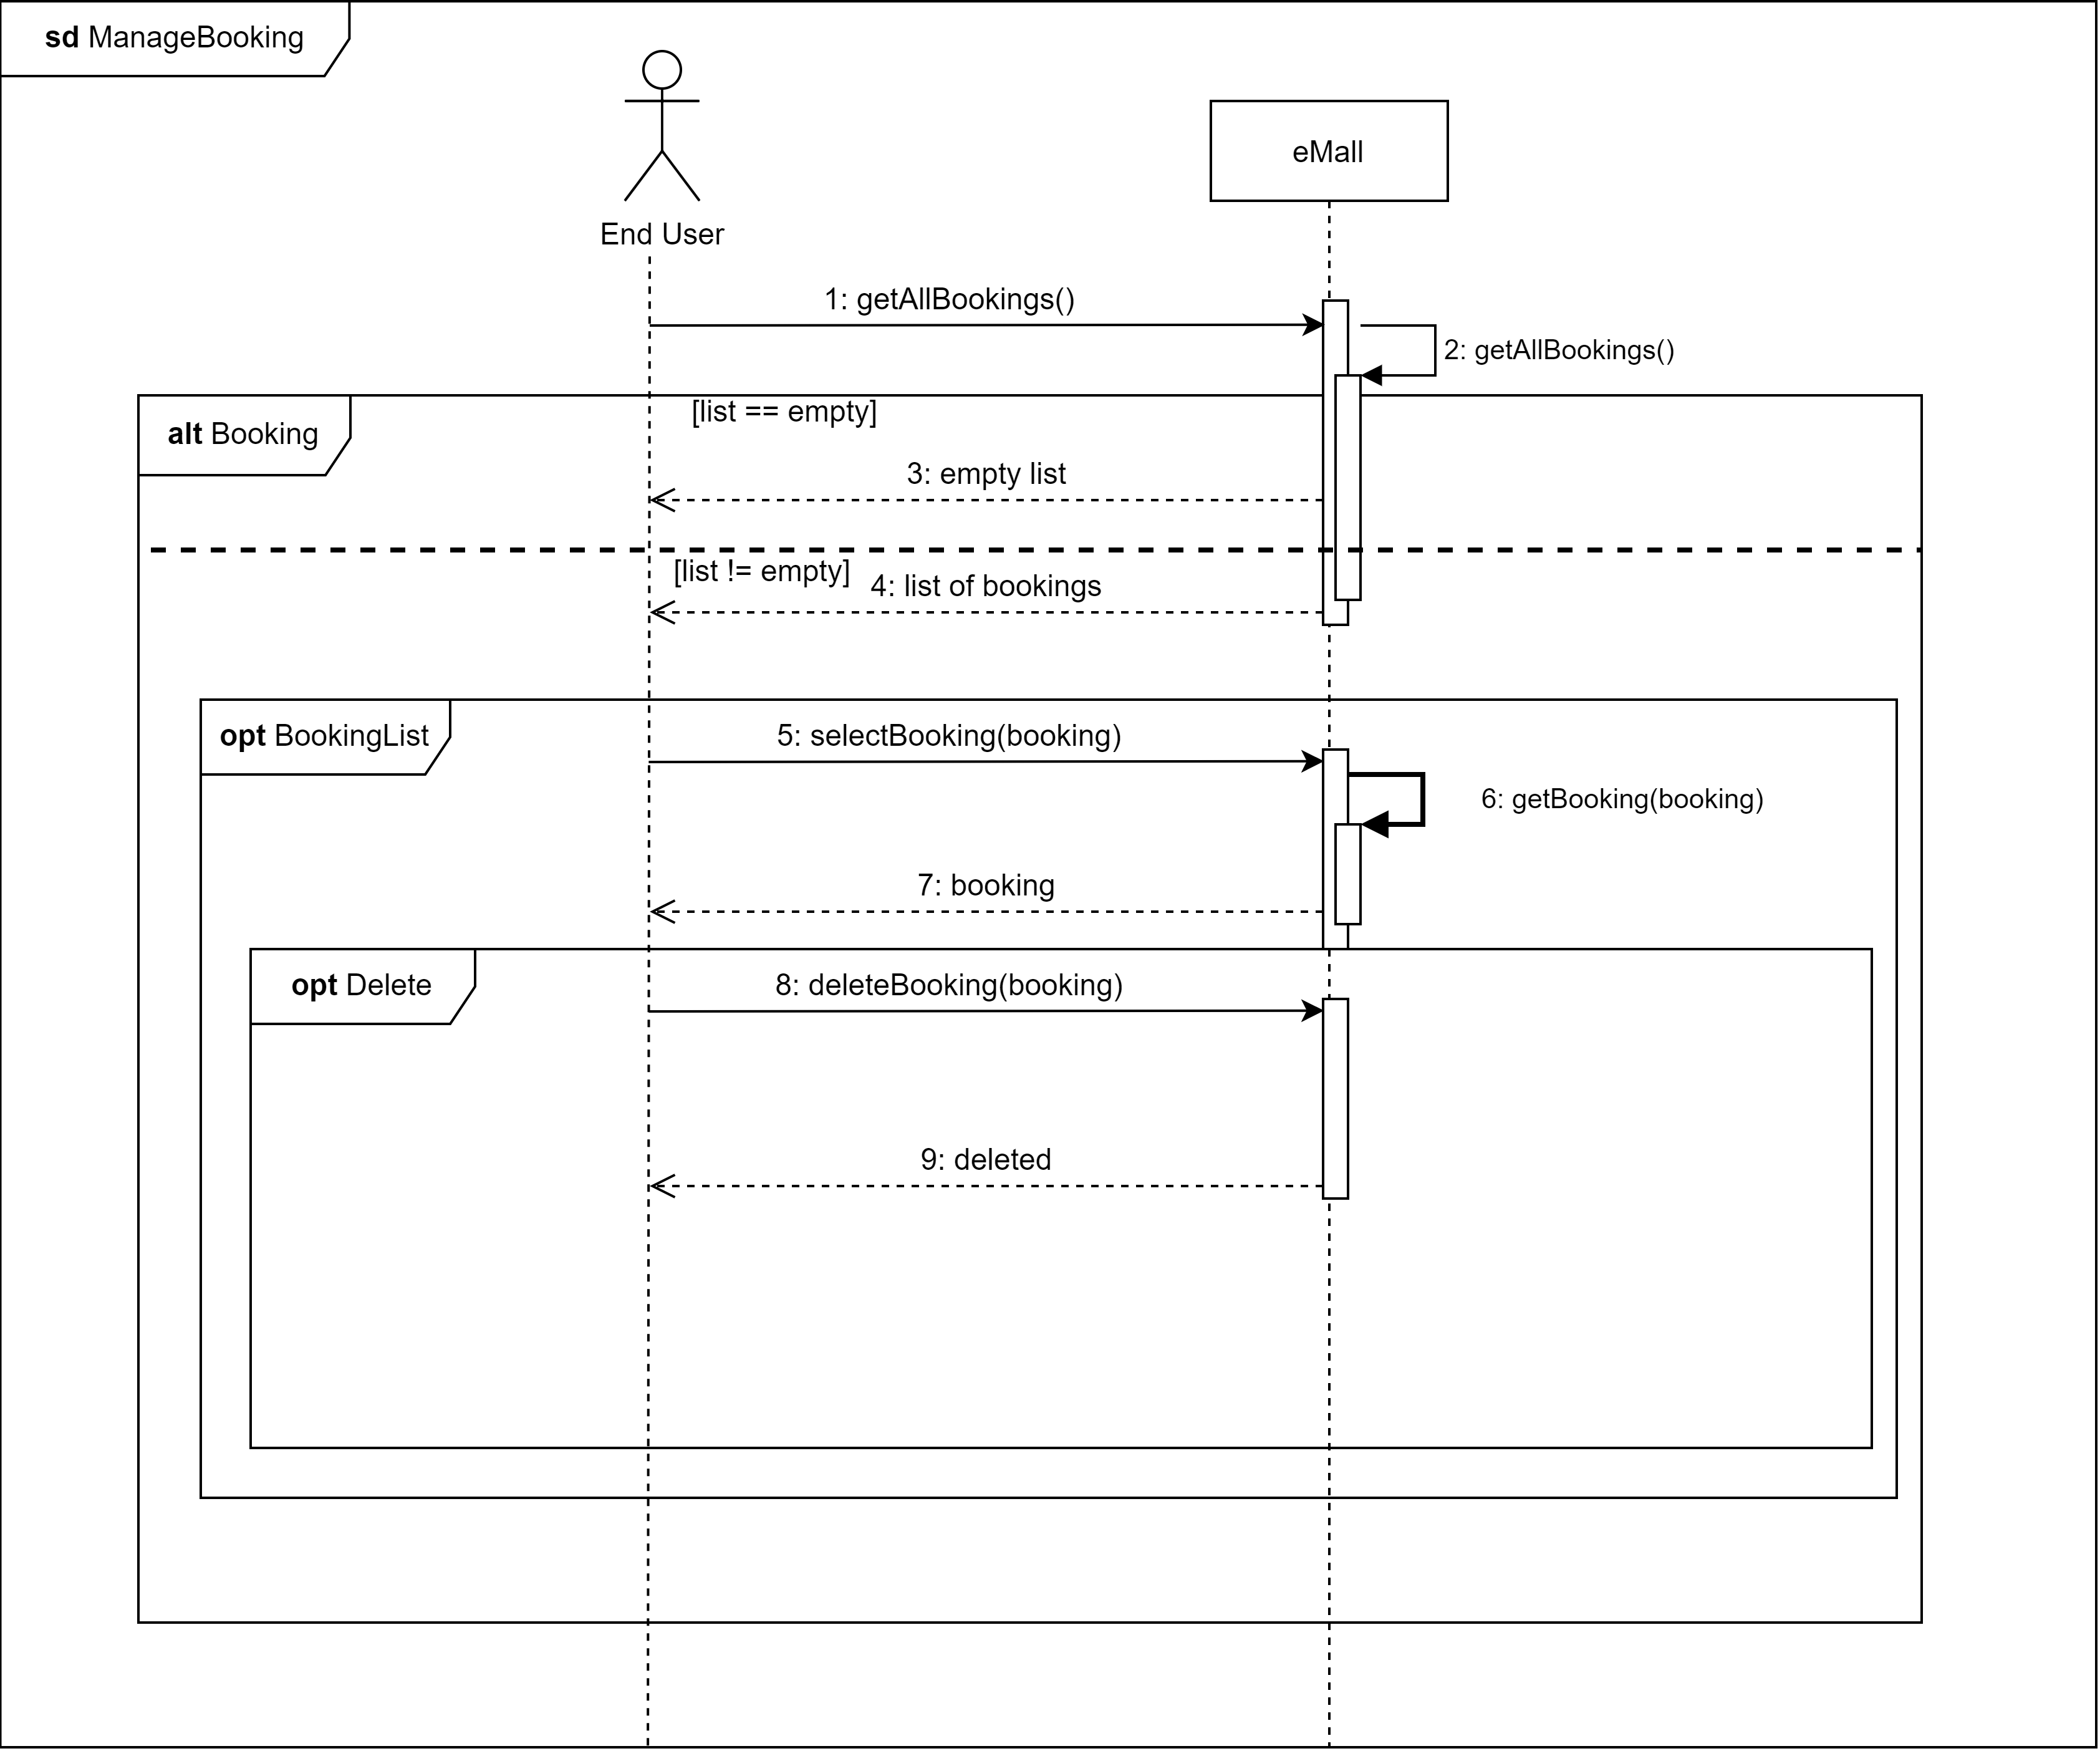
\includegraphics[width=\textwidth]{images/sd_manageBooking.png}
    \caption{End user managing booking sequence diagram.}
    \label{fig:sd_manage_booking}
\end{figure}
\begin{figure}[H]
    \centering
    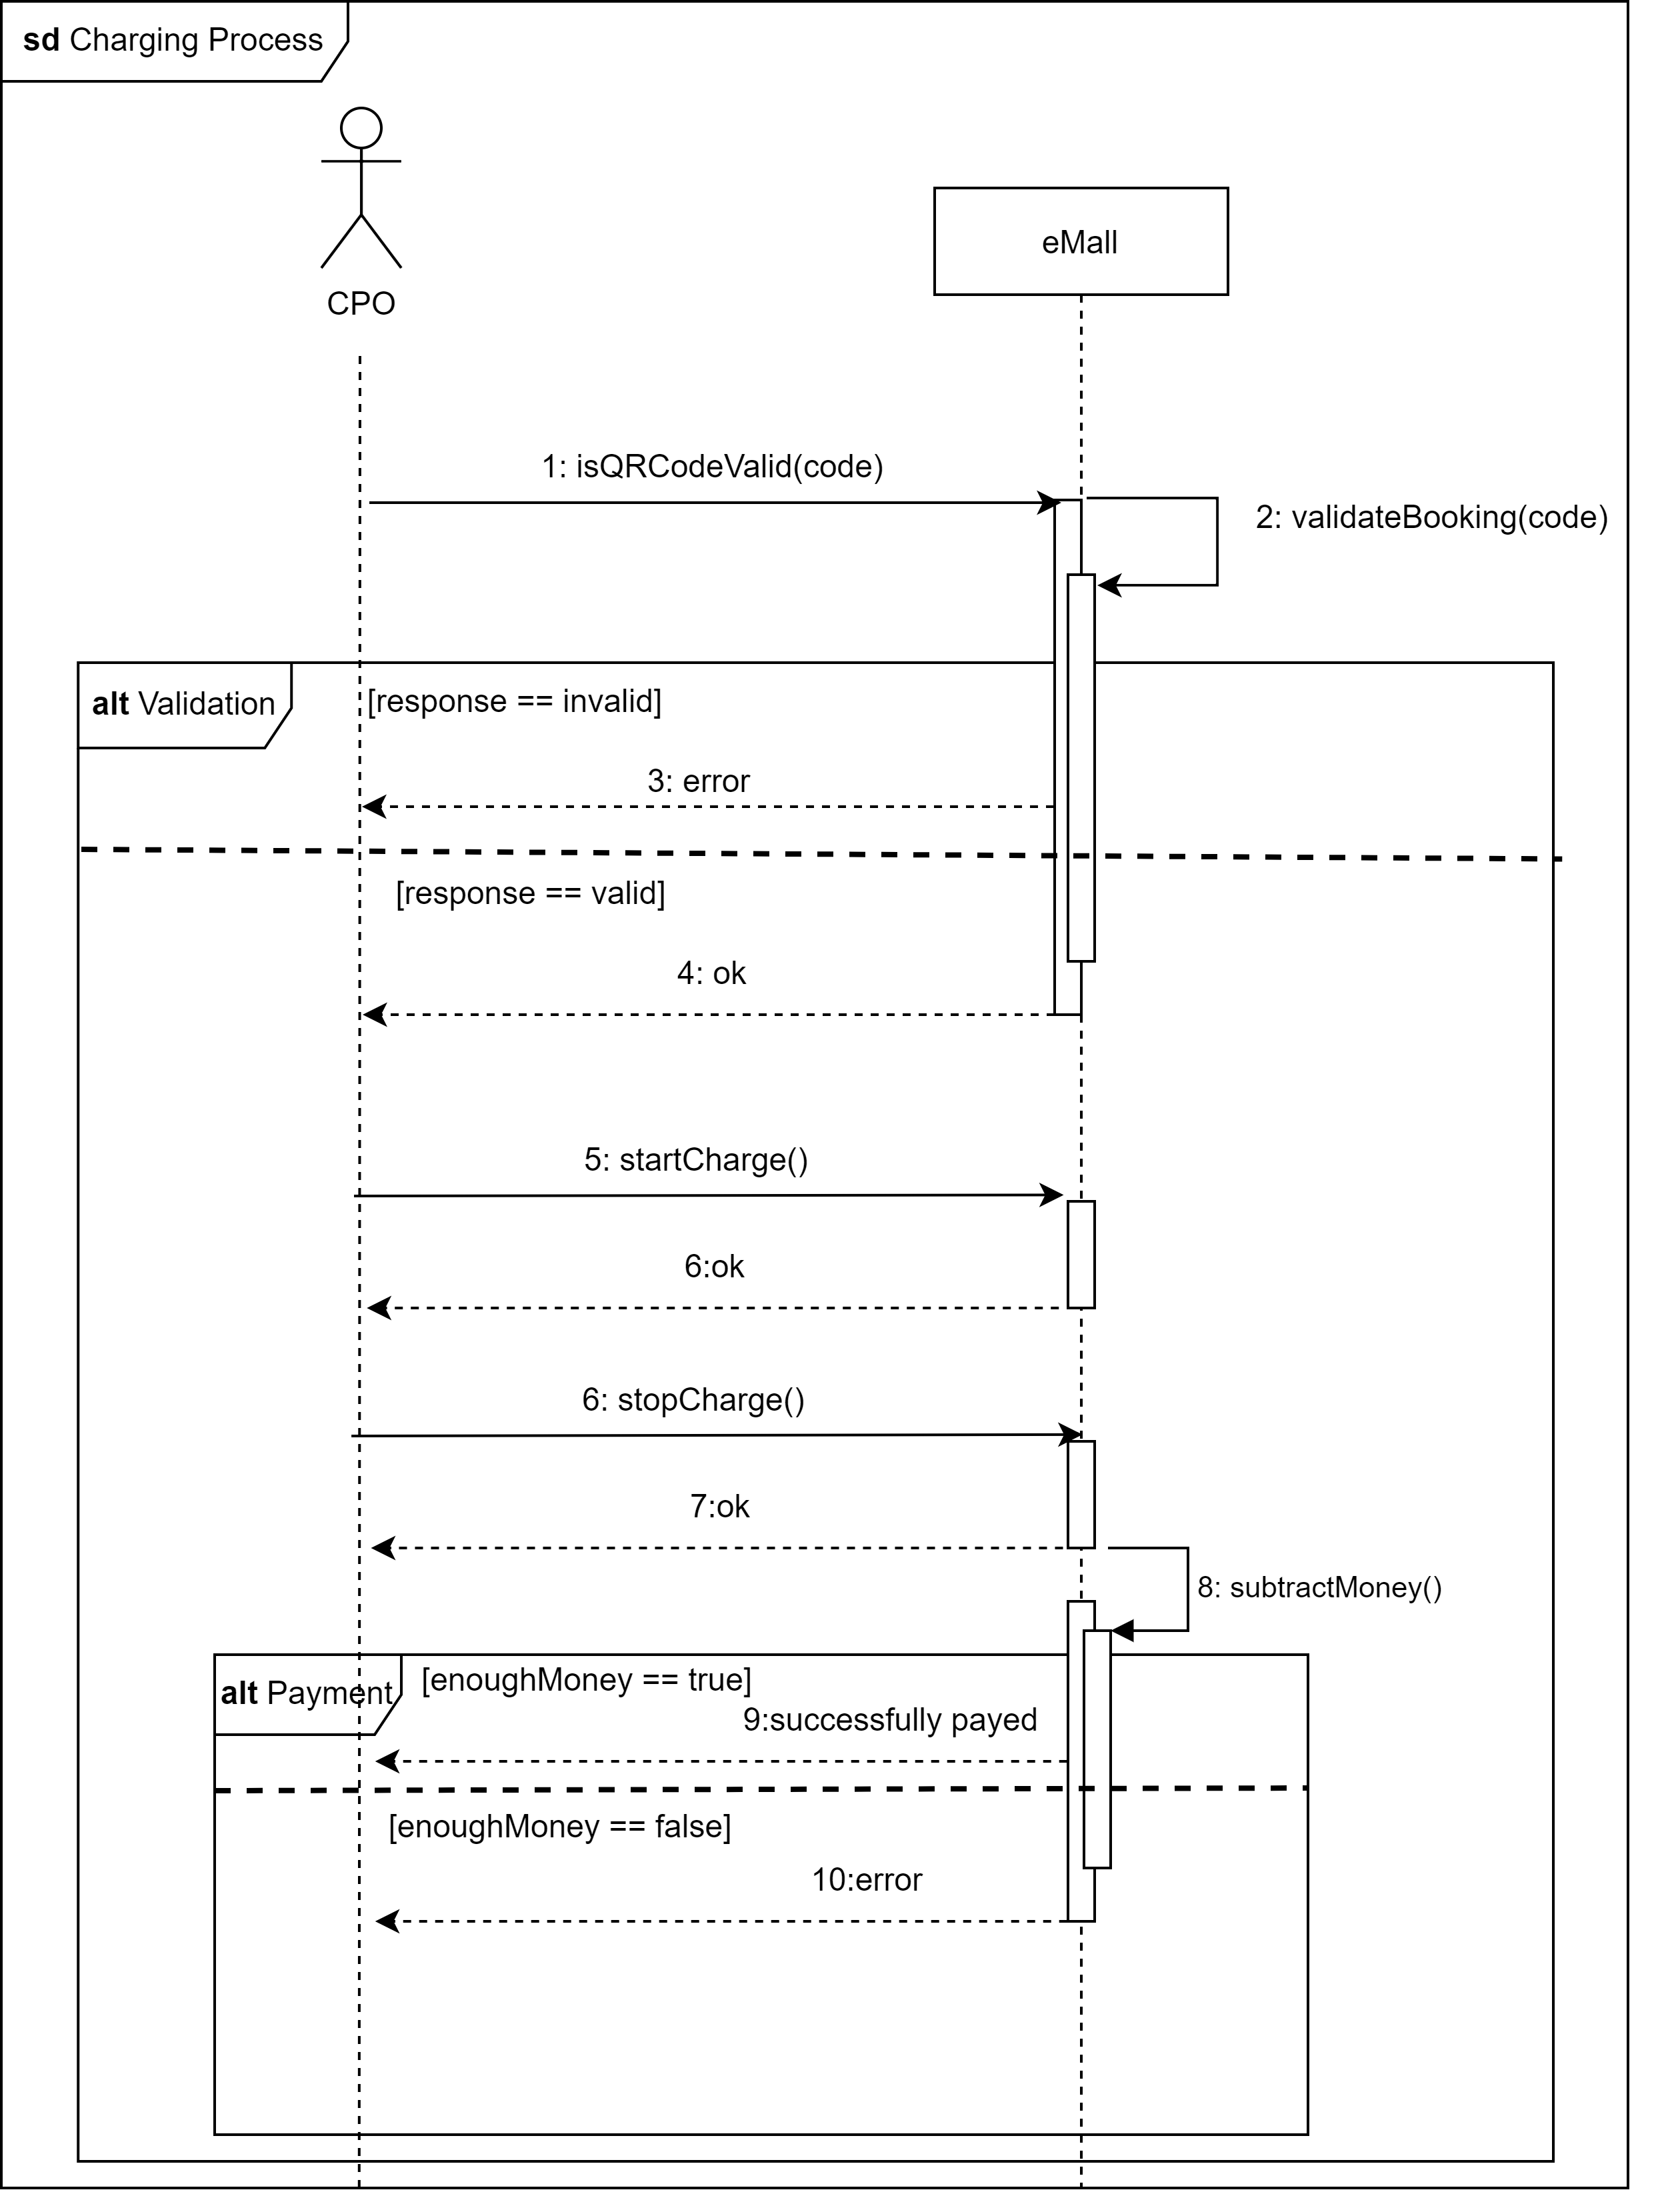
\includegraphics[width=\textwidth]{images/sd_scan.png}
    \caption{Charging process sequence diagram.}
    \label{fig:sd_charging_process}
\end{figure}
\begin{figure}[H]
    \centering
    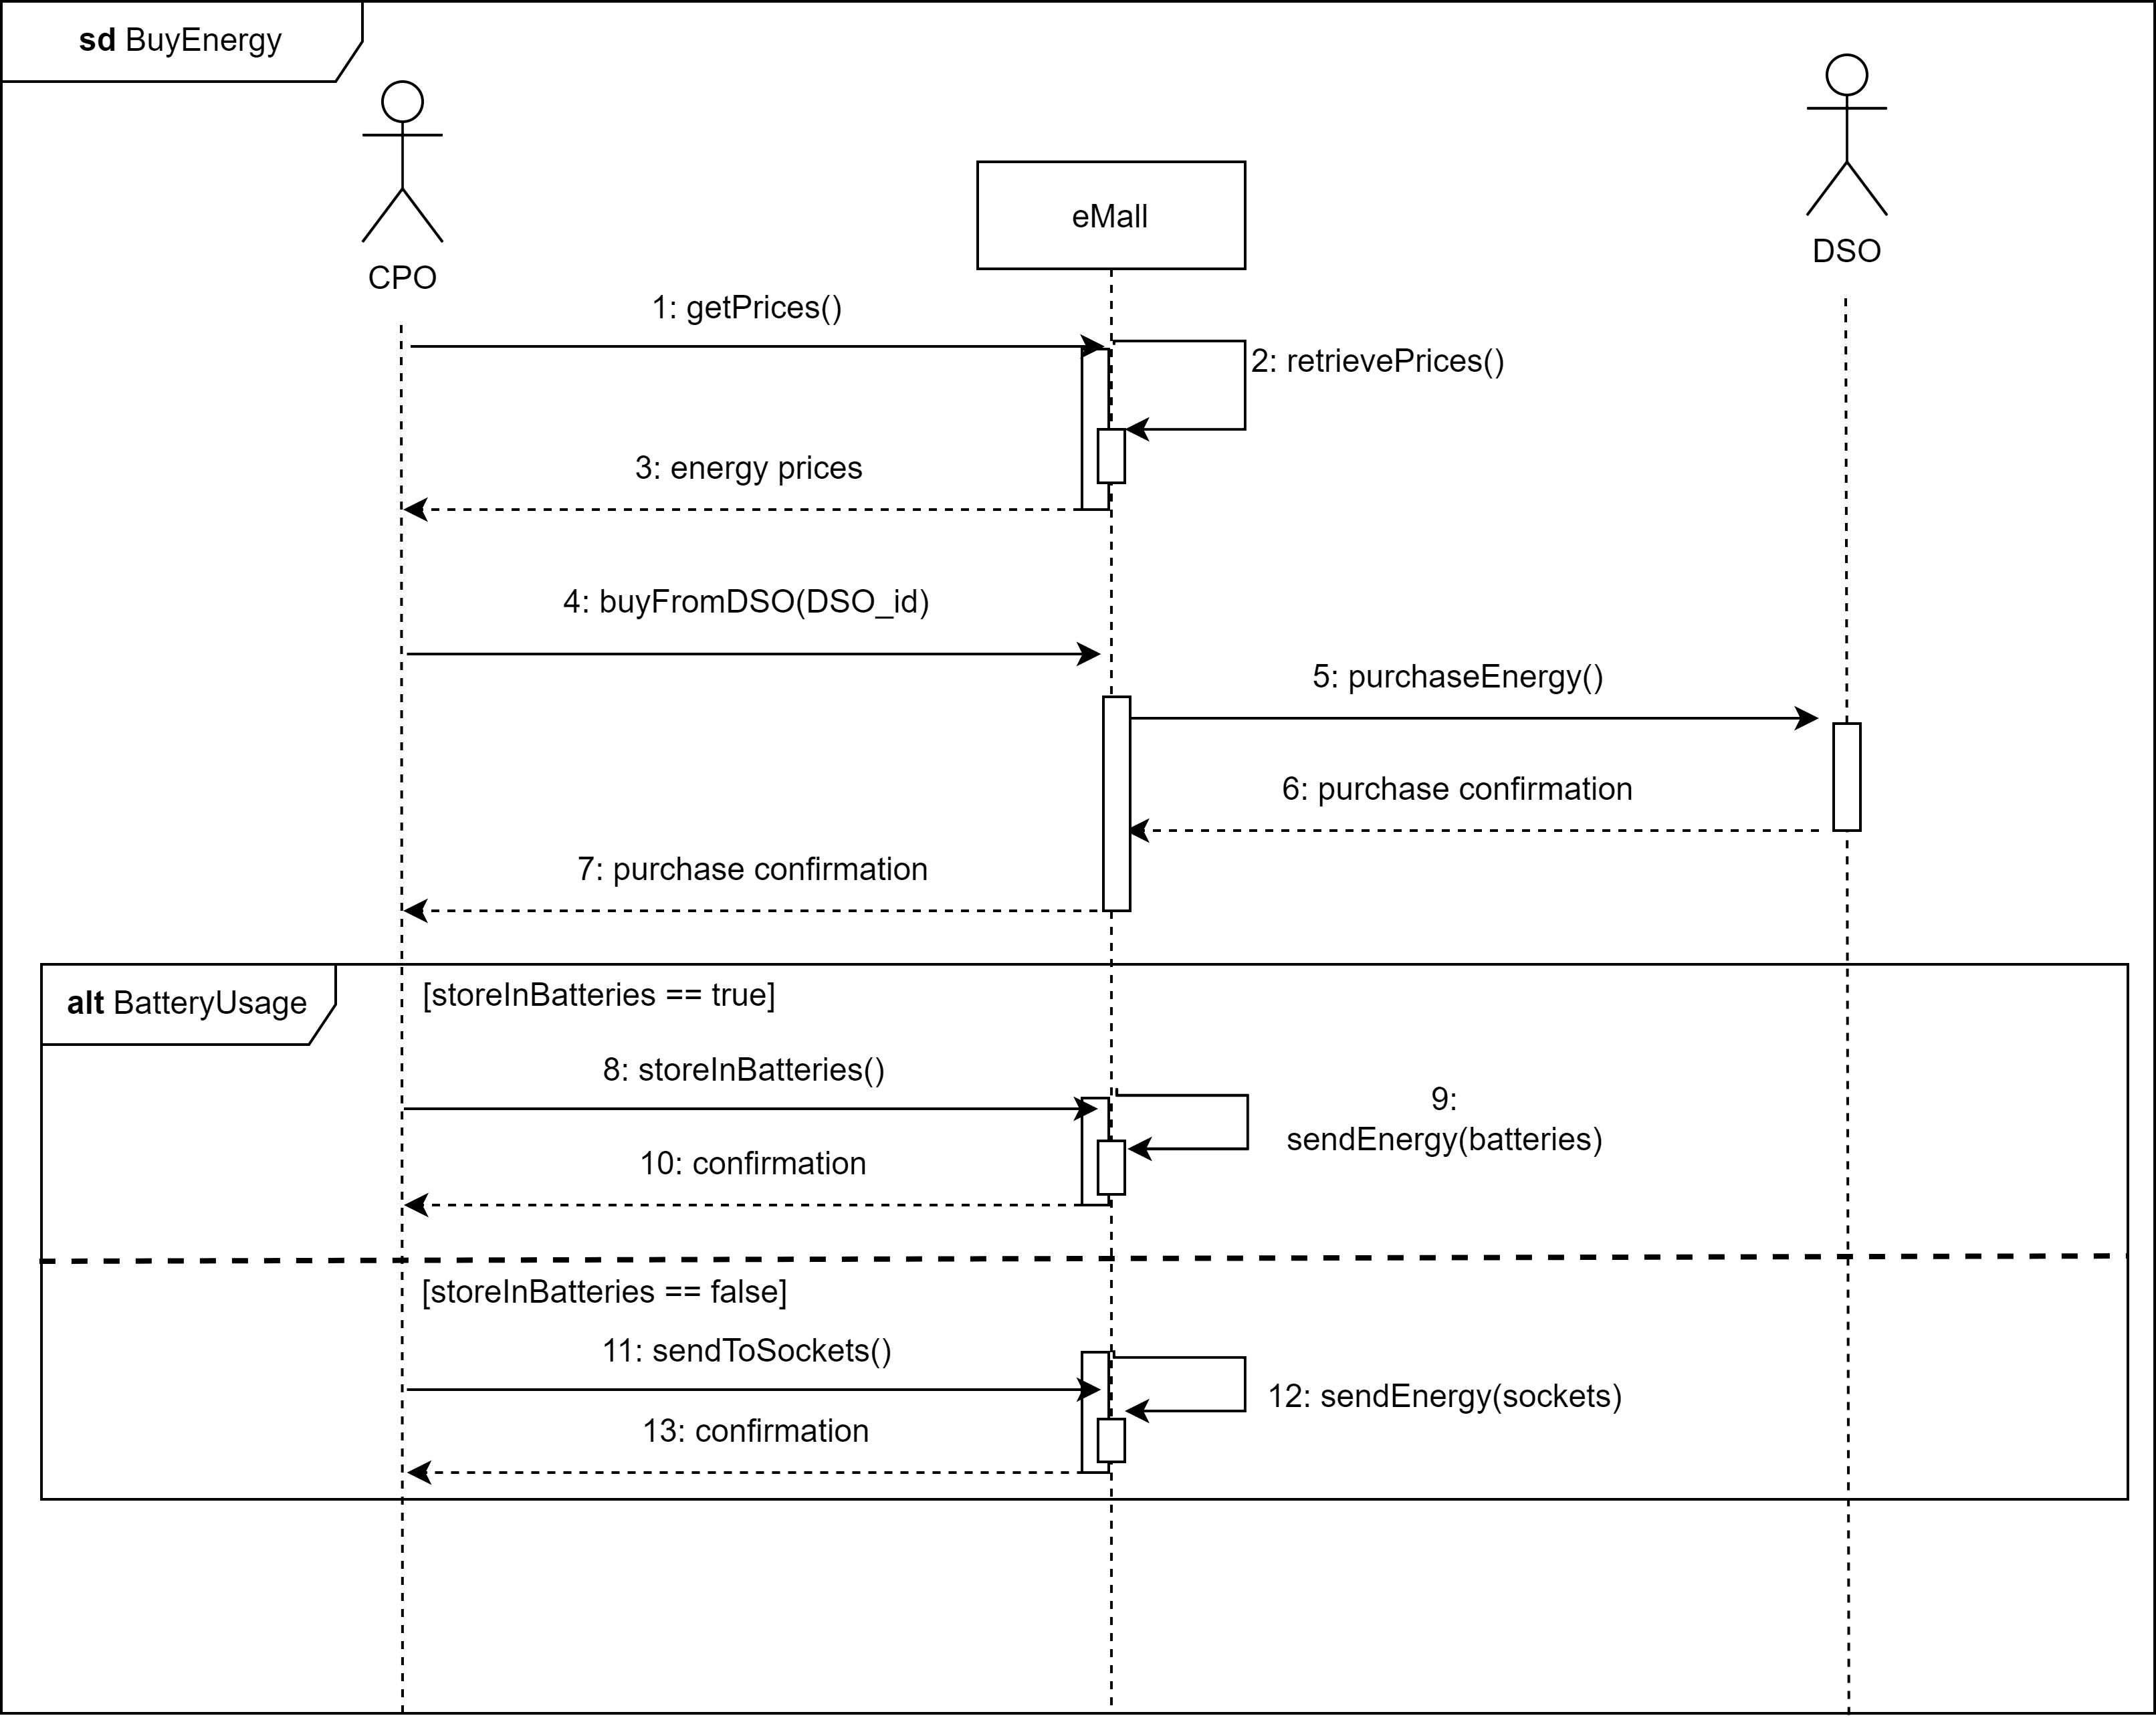
\includegraphics[width=\textwidth]{images/sd_buy.png}
    \caption{CPO puchasing energy sequence diagram.}
    \label{fig:sd_cpo_purchasing_energy}
\end{figure}
\begin{figure}[H]
    \centering
    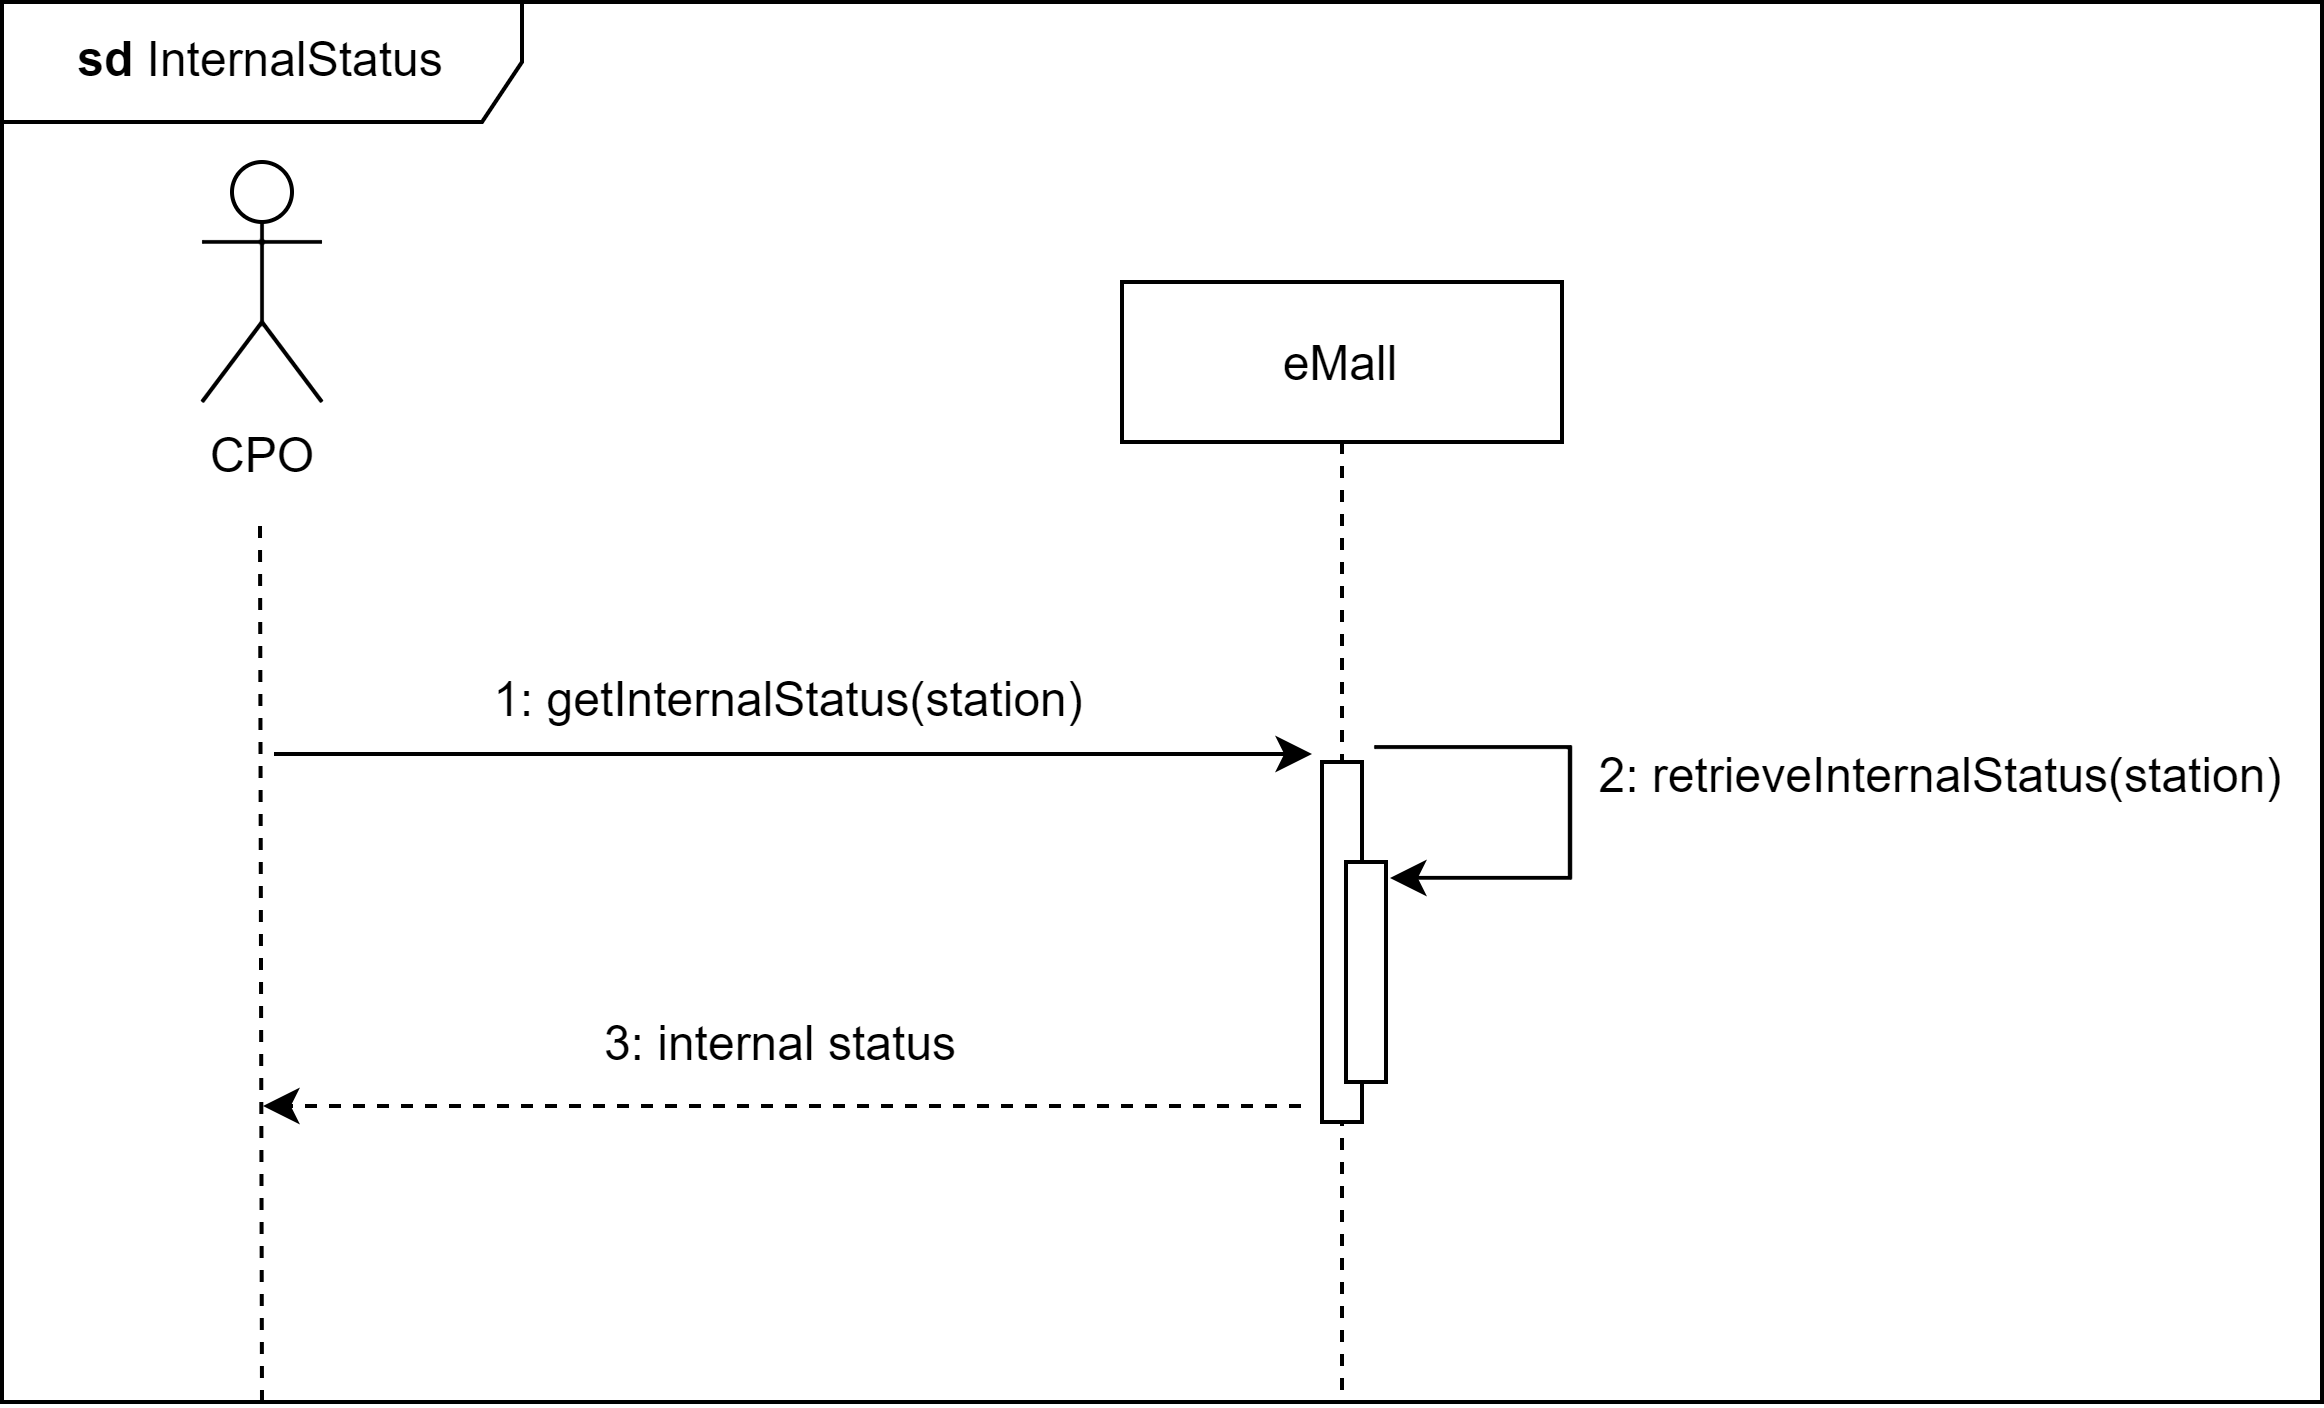
\includegraphics[width=\textwidth]{images/sd_internal.png}
    \caption{Internal status sequence diagram.}
    \label{fig:sd_internal_status}
\end{figure}
\begin{figure}[H]
    \centering
    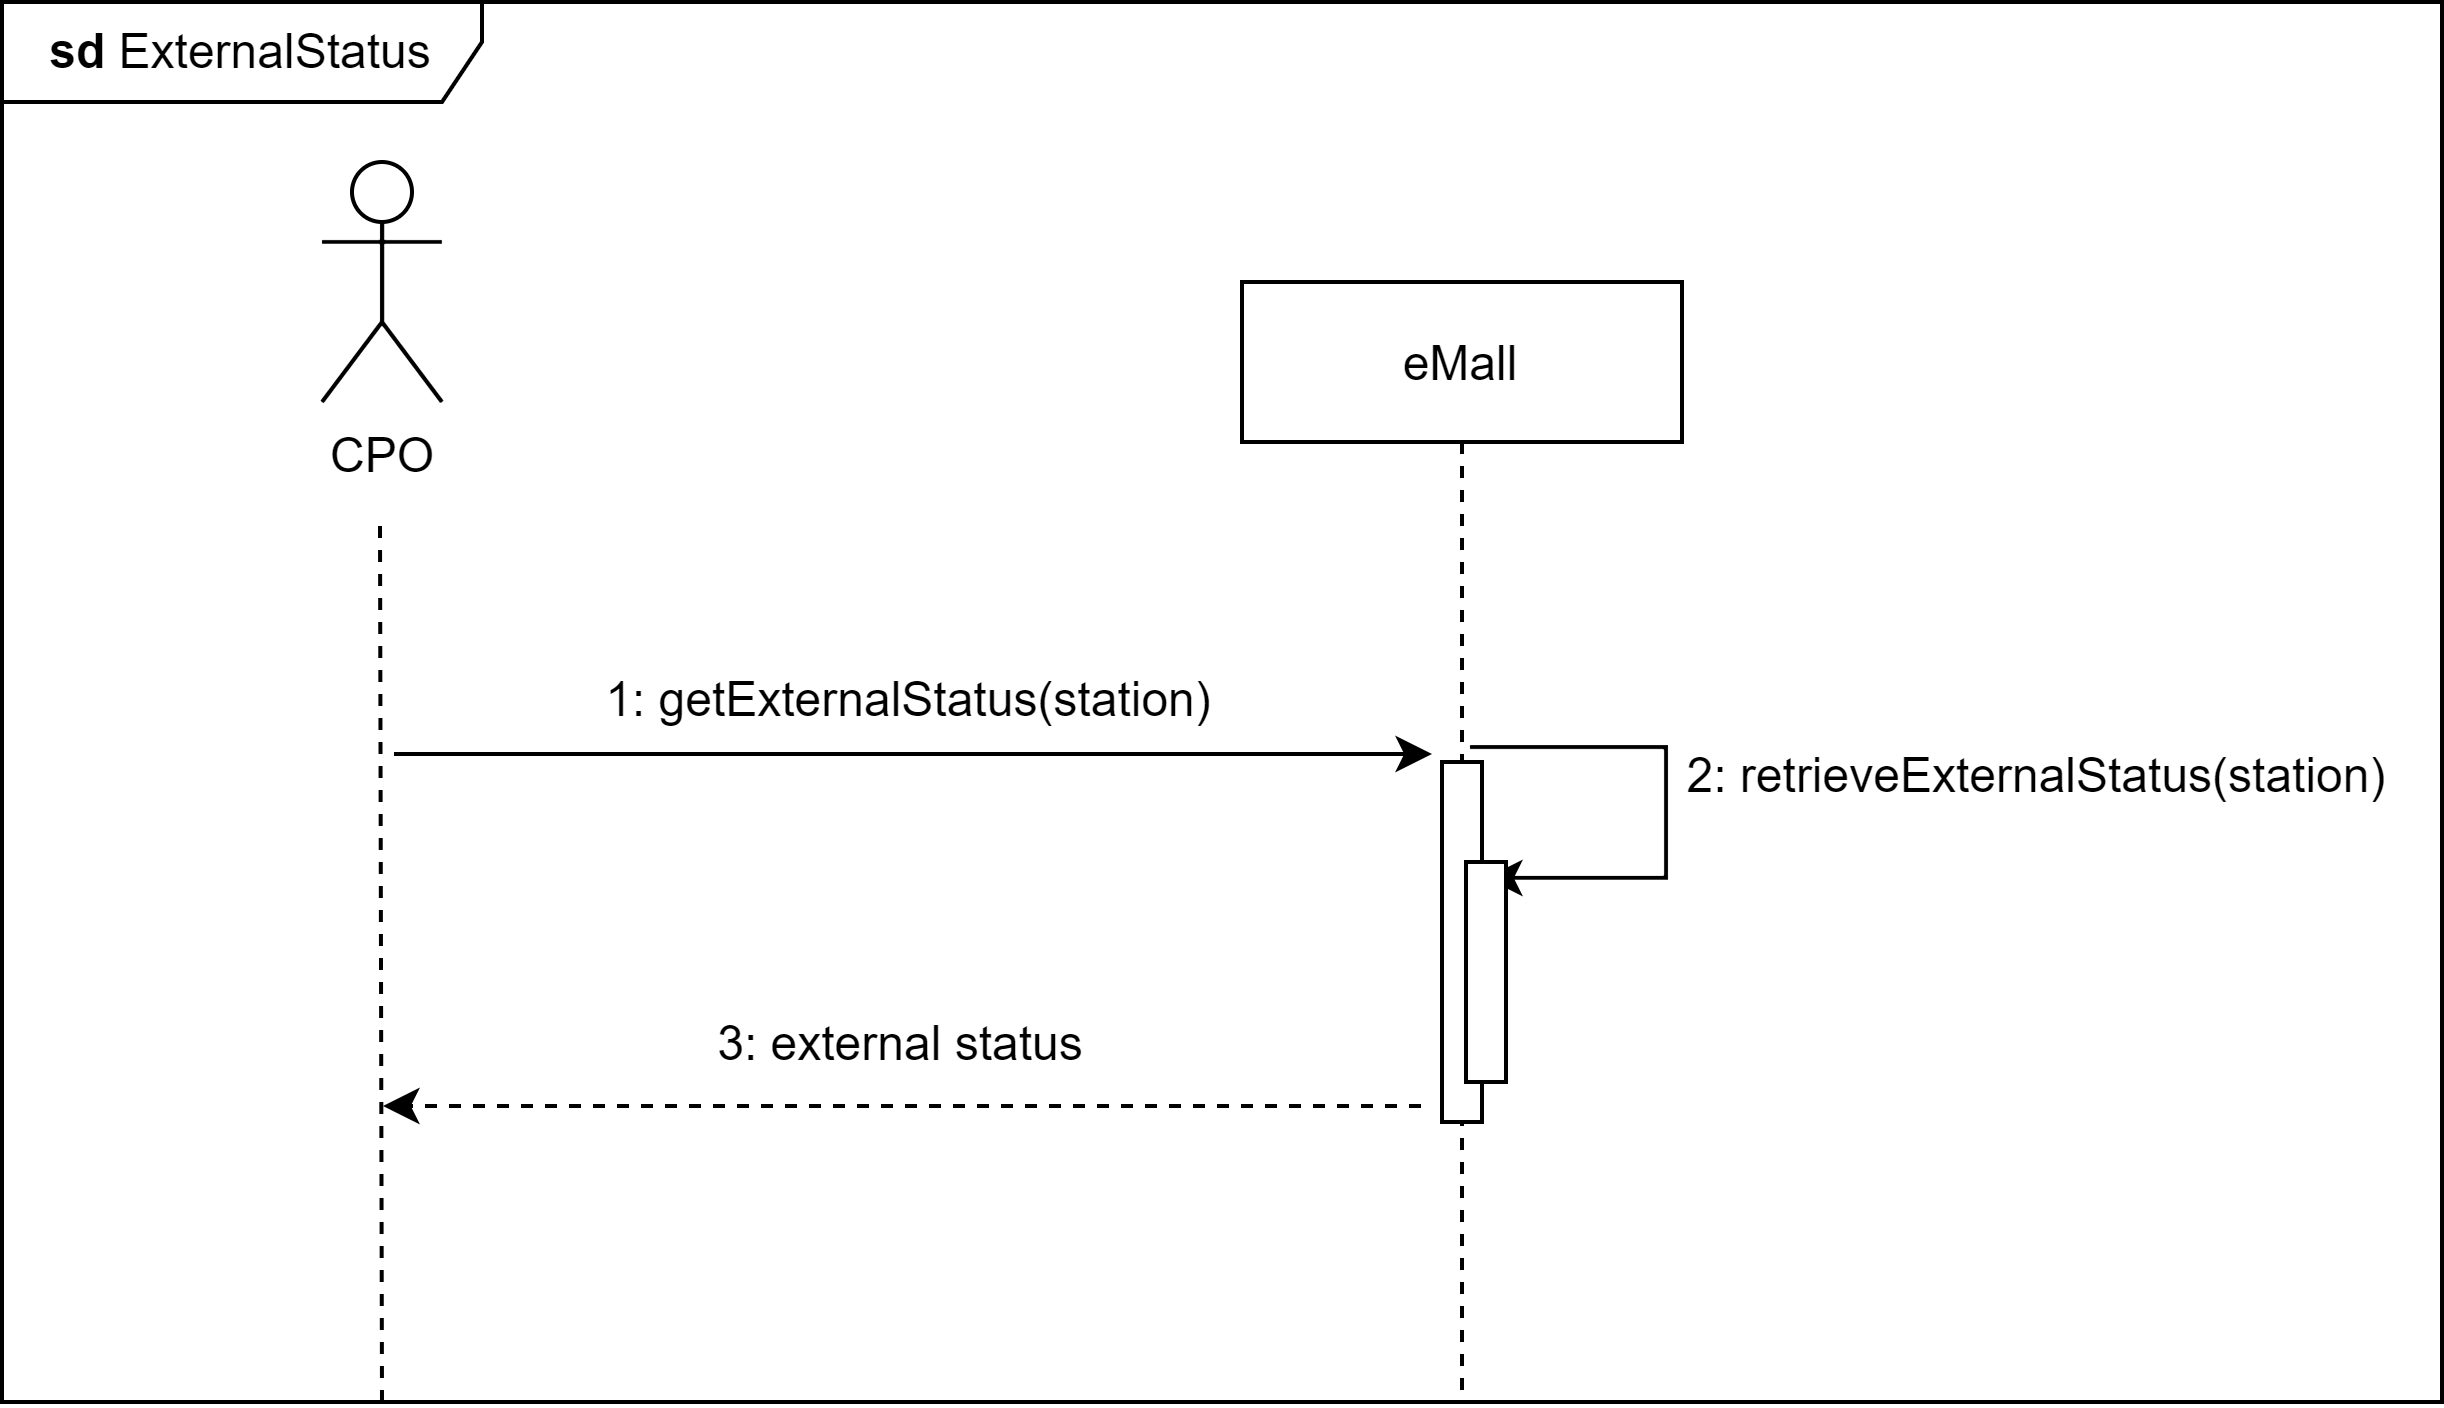
\includegraphics[width=\textwidth]{images/sd_external.png}
    \caption{External status sequence diagram.}
    \label{fig:sd_external_status}
\end{figure}
\begin{figure}[H]
    \centering
    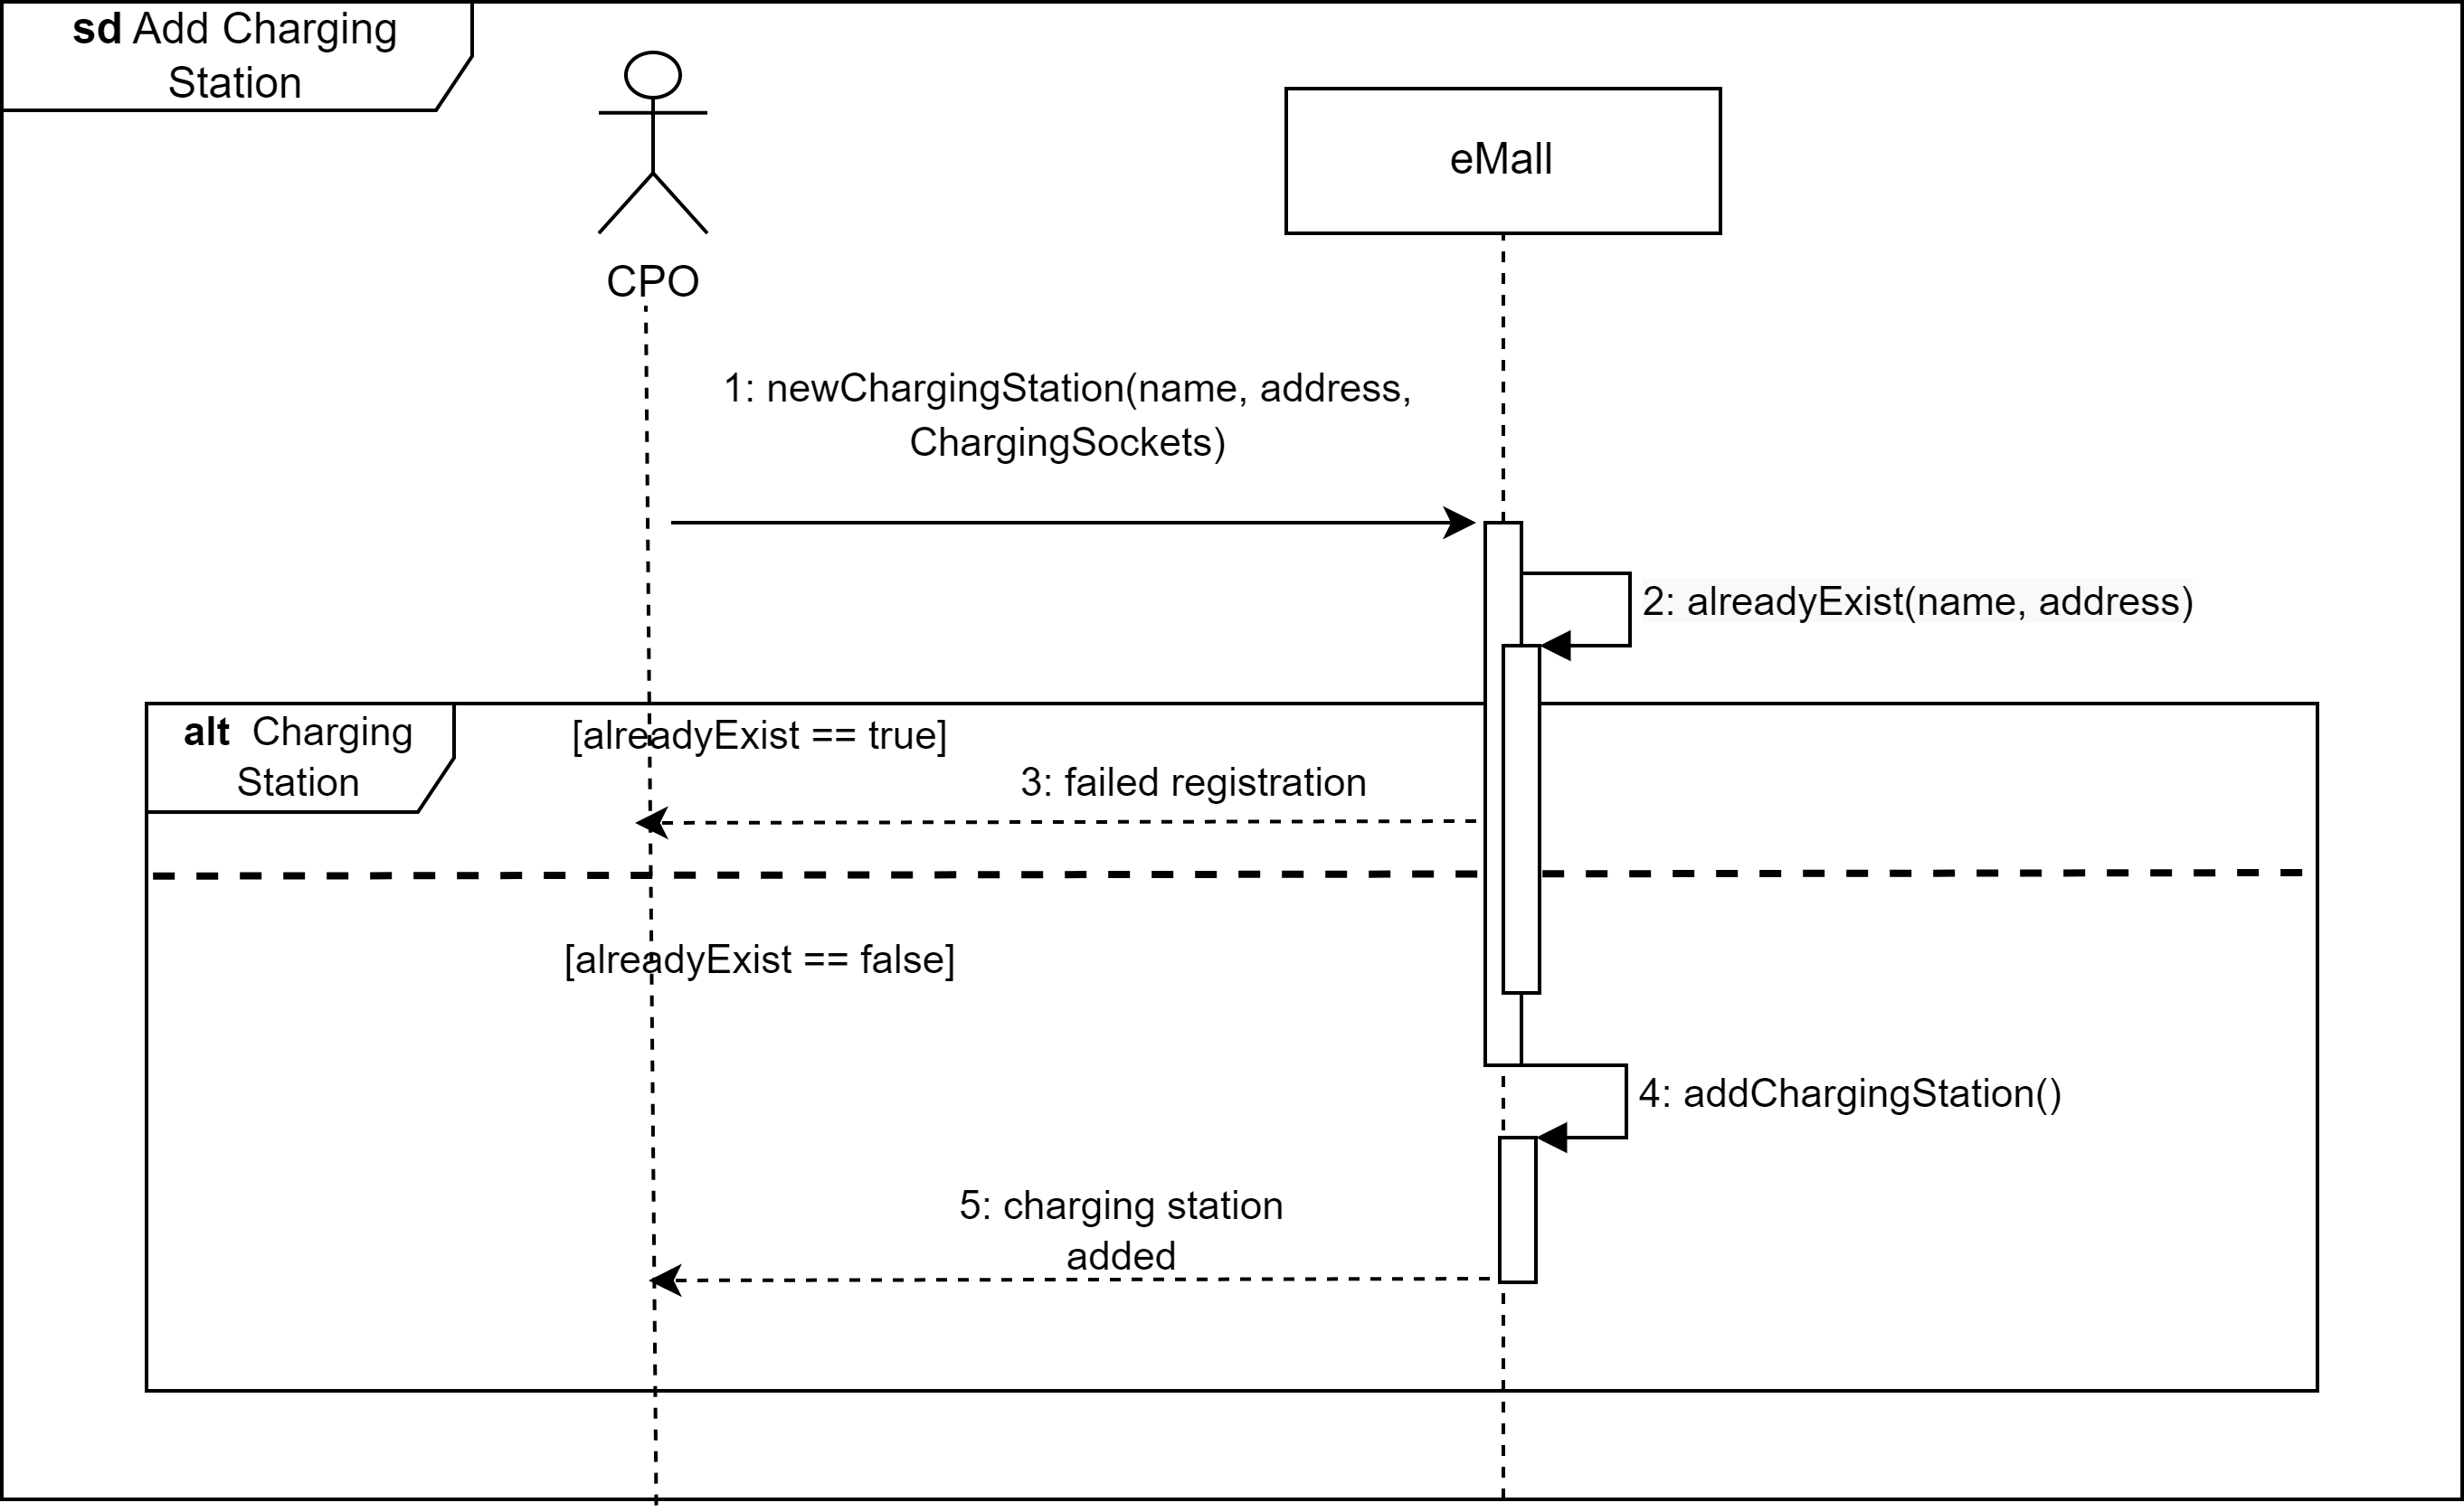
\includegraphics[width=\textwidth]{images/sd_add_station.png}
    \caption{Add charging station sequence diagram.}
    \label{fig:sd_add_charging_station}
\end{figure}
\subsubsection{List of functional requirements}
\begin{longtable}{|c|l|}
\hline
\rowcolor[HTML]{B8C8D5} 
{\color[HTML]{000000} \textbf{Requirements}} & \multicolumn{1}{c|}{\cellcolor[HTML]{B8C8D5}{\color[HTML]{000000} \textbf{Description}}} \\ \hline
\endfirsthead
%
\endhead
%
R.1 \label{R.1}& \begin{tabular}[c]{@{}l@{}}The system must allow the end user to register himself to the system \\ by providing all the mandatory information.\end{tabular} \\ \hline
R.2 \label{R.2}& \begin{tabular}[c]{@{}l@{}}The system must allow the end user to register a payment method.\end{tabular} \\ \hline
R.3 \label{R.3}& \begin{tabular}[c]{@{}l@{}}The system must verify the uniqueness of the mail and username \\ of the end user to be registered.\end{tabular} \\ \hline
R.4 \label{R.4}& \begin{tabular}[c]{@{}l@{}}The system must send a confirmation on the end user's email after \\ his registration.\end{tabular} \\ \hline
R.5 \label{R.5}& \begin{tabular}[c]{@{}l@{}}The system must allow the end user to log into their account by \\ entering their username and password.\end{tabular} \\ \hline
R.6 \label{R.6}& \begin{tabular}[c]{@{}l@{}}The system must allow the end user to book a charging socket of a \\ certain charging station in a specific time slot.\end{tabular} \\ \hline
R.7 \label{R.7}& The system must generate a QR-Code after the end user's reservation. \\ \hline
R.8 \label{R.8}& The system must show to the end user the suggested charging stations. \\ \hline
R.9 \label{R.9}& \begin{tabular}[c]{@{}l@{}}The system must show to the end user the available and unavailable\\ time slots of a certain charging socket.\end{tabular} \\ \hline
R.10 \label{R.10}& The system must access to the end user's location through GPS. \\ \hline
R.11 \label{R.11}& The system must access to the end user's calendar. \\ \hline
R.12 \label{R.12}& The system must access to the end user's vehicle status battery. \\ \hline
R.13 \label{R.13}& The system must allow the end user to delete his reservation. \\ \hline
R.14 \label{R.14}& \begin{tabular}[c]{@{}l@{}}The system must notify the end user when the charge of his vehicle\\ is completed.\end{tabular} \\ \hline
R.15 \label{R.15}& \begin{tabular}[c]{@{}l@{}}The system must subtract the cost of the charge from end user's \\ payment method.\end{tabular} \\ \hline
R.16 \label{R.16}& \begin{tabular}[c]{@{}l@{}}The system must send to the end user an email with the invoice for\\ the used service.\end{tabular} \\ \hline
R.17 \label{R.17}& \begin{tabular}[c]{@{}l@{}}The system must allow the end user to book a time slot.\end{tabular} \\ \hline
R.18 \label{R.18}& \begin{tabular}[c]{@{}l@{}}The system must stop the charge when the upper bound of time slot\\ is exceeded.\end{tabular} \\ \hline
R.19 \label{R.19}& The system must allow the end user to see his current bookings. \\ \hline
R.20 \label{R.20}& \begin{tabular}[c]{@{}l@{}}The system must allow the end user to search for a certain charging\\ station.\end{tabular} \\ \hline
R.21 \label{R.21}& The system must allow the end user to stop the charging process. \\ \hline
R.22 \label{R.22}& The system must allow the end user to start the charging process. \\ \hline
R.23 \label{R.23}& The system must allow the end user to monitor the charging process. \\ \hline
R.24 \label{R.24}& \begin{tabular}[c]{@{}l@{}}The system must prevent the end user from reserving a charging \\socket in a certain time slot, if he already has another reservation \\in that time slot.\end{tabular} \\ \hline
R.25 \label{R.25}& \begin{tabular}[c]{@{}l@{}}The system must prevent at least two different end users from \\reserving the same charging socket in the same time slot.\end{tabular} \\ \hline
%
R.26 \label{R.26}& \begin{tabular}[c]{@{}l@{}}The system must allow the CPO to register himself to the system \\ by providing all the mandatory and commercial information.\end{tabular} \\ \hline
R.27 \label{R.27}& \begin{tabular}[c]{@{}l@{}}The system must verify the uniqueness of the mail of the CPO to\\ be registered.\end{tabular} \\ \hline
R.28 \label{R.28}& The system must verify the correctness of the CPO's commercial data. \\ \hline
R.29 \label{R.29}& \begin{tabular}[c]{@{}l@{}}The system must send a confirmation on the CPO's email after \\ his registration.\end{tabular} \\ \hline
R.30 \label{R.30}& \begin{tabular}[c]{@{}l@{}}The system must allow the CPO to log into their account by \\ entering their username and password.\end{tabular} \\ \hline
R.31 \label{R.31}& \begin{tabular}[c]{@{}l@{}}The system must allow the CPO to know the internal and external\\ status of charging sockets of his charging stations.\end{tabular} \\ \hline
R.32 \label{R.32}& The system must allow the CPO to monitor the charging process. \\ \hline
R.33 \label{R.33}& \begin{tabular}[c]{@{}l@{}}The system must allow the CPO to acquire information about \\ the price of energy from DSOs.\end{tabular} \\ \hline
R.34 \label{R.34}& The system must allow the CPO to acquire energy from DSOs. \\ \hline
R.35 \label{R.35}& \begin{tabular}[c]{@{}l@{}}The system must allow the CPO to decide whether to store or not\\ energy.\end{tabular} \\ \hline
R.36 \label{R.36}& \begin{tabular}[c]{@{}l@{}}The system must allow the CPO to decide whether to use available\\ energy in the batteries.\end{tabular} \\ \hline
R.37 \label{R.37}& \begin{tabular}[c]{@{}l@{}}The system must forbid to charge the vehicle to a user that scans\\ a QR-Code which is not valid (expired, wrong etc.).\end{tabular} \\ \hline
R.38 \label{R.38}& \begin{tabular}[c]{@{}l@{}}The system must indicate whether a slot is booked or not, and it must\\ forbid to book an already booked time slot.\end{tabular} \\ \hline
R.39 \label{R.39}& \begin{tabular}[c]{@{}l@{}}The system must manage the concurrent booking of a slot: if a\\ user waits too much to book a slot and meanwhile another user\\ books that slot, the system must notify the first user when he tries \\to perform the booking.\end{tabular} \\ \hline
R.40 \label{R.40}& \begin{tabular}[c]{@{}l@{}}The system must allow the CPO to add a new charging station.
\end{tabular} \\ \hline
R.41 \label{R.41}& \begin{tabular}[c]{@{}l@{}}The system must allow the CPO to view, via the CPMS, the \\ charge percentage of the battery cluster. \end{tabular} \\ \hline
R.42 \label{R.42}& \begin{tabular}[c]{@{}l@{}}If the user initiates charging and there is not enough charge in the\\ battery cluster, the system, to avoid service disruption, allows the \\charging station to receive power directly from the DSO channel. \end{tabular} \\ \hline
\end{longtable}
\clearpage
\subsection{Mapping on requirements}
% Please add the following required packages to your document preamble:
% \usepackage[table,xcdraw]{xcolor}
% If you use beamer only pass "xcolor=table" option, i.e. \documentclass[xcolor=table]{beamer}
\begin{table}[H]
\resizebox{\textwidth}{!}{%
\begin{tabular}{|l|l|l|}
\hline
\rowcolor[HTML]{B8C8D5} 
\multicolumn{1}{|c|}{\cellcolor[HTML]{B8C8D5}\textbf{Goals}} & \multicolumn{1}{c|}{\cellcolor[HTML]{B8C8D5}\textbf{Domain Assumptions}} & \multicolumn{1}{c|}{\cellcolor[HTML]{B8C8D5}{\color[HTML]{000000} \textbf{Requirements}}} \\ \hline
G.1 &  D.1, D.2, D.3, D.4, D.5, D.12, D.15 & \begin{tabular}[c]{@{}l@{}}R.1, R.3, R.4, R.5, R.8, R.10, R.11, \\R.12, R.20, R.24, R.25 \end{tabular}\\ \hline
G.2 &  D.1, D.3, D.14, D.15, D.17 & \begin{tabular}[c]{@{}l@{}} R.1, R.3, R.4, R.5, R.6, R.7, R.9, R.13,\\ R.17, R.19, R.38, R.39 \end{tabular}\\ \hline
G.3 & D.1, D.3, D.6, D.7, D.8, D.15, D.18 & \begin{tabular}[c]{@{}l@{}} R.1, R.3, R.4, R.5, R.14, R.18, R.21,\\ R.22, R.23, R.37 \end{tabular}\\ \hline
G.4 & D.1, D.3, D.15, D.24, D.26 & \begin{tabular}[c]{@{}l@{}} R.1, R.2, R.3, R.4, R.5, R.15, R.16 \end{tabular}\\ \hline
G.5 &\begin{tabular}[c]{@{}l@{}} D.9, D.10, D.11, D.12, D.13, D.16,\\ D.19, D.20, D.22, D.23, D.28, D.29, D.30\end{tabular} & \begin{tabular}[c]{@{}l@{}}R.26, R.27, R.28, R.29, R.30, R.31,\\ R.32, R.40, R.41, R.42 \end{tabular}\\ \hline
G.6 & D.9, D.10, D.11, D.16, D.21, D.28, D.29, D.30 &\begin{tabular}[c]{@{}l@{}} R.26, R.27, R.28, R.29, R.33, R.34 \end{tabular}\\ \hline
G.7 & D.9, D.10, D.11, D.13, D.15, D.25, D.27, D.28, D.29, D.30 & \begin{tabular}[c]{@{}l@{}} R.26, R.27, R.28, R.29, R.35, R.36, \\ R.42\end{tabular}\\ \hline
\end{tabular}
}
\end{table}
\textbf{Why this mapping?} The table above reports the mapping of assuptions and requirements on the goals. It is useful so that you have a clear and immediate idea about which goals are involved in a certain assumption or requirement. In general, we have a division between the end user related goals (G1, G2, G3, G4) and the CPO goals (G5, G6, G7). As we can see from the table above some requirements / assumption are repeated, this is because some of them are essential for all the goals, for example the end user login or the CPO login.
\subsection{Traceability matrix}
\begin{longtable}{|l|l|l|l|}
\hline
\rowcolor[HTML]{B8C8D5} 
Raw ID & Goal ID & Req ID & Use Case ID \\ \hline
\endfirsthead
%
\endhead
%
r1     & G.1     & R.1    &       UC.1      \\ \hline
r2     & G.1     & R.3    &       UC.1      \\ \hline
r3     & G.1     & R.4    &       UC.1    \\ \hline
r4    & G.1     & R.5    &       UC.2    \\ \hline
r5     & G.1     & R.8    &       UC.3    \\ \hline
r6     & G.1     & R.9    &       UC.3    \\ \hline
r7     & G.1     & R.10   &         UC.3    \\ \hline
r8     & G.1     & R.11   &         UC.3    \\ \hline
r9     & G.1     & R.12   &         UC.3    \\ \hline
r10     & G.1     & R.20   &         UC.3    \\ \hline
r11    & G.1     & R.24   &         UC.3    \\ \hline
r12    & G.1     & R.25   &         UC.3    \\ \hline

r13    & G.2     & R.1    &         UC.1    \\ \hline
r14    & G.2     & R.3    &         UC.1    \\ \hline
r15    & G.2     & R.4    &         UC.1    \\ \hline
r16    & G.2     & R.5    &         UC.2    \\ \hline
r17    & G.2     & R.6    &         UC.3    \\ \hline
r18    & G.2     & R.7    &         UC.3    \\ \hline
r19    & G.2     & R.9    &         UC.3    \\ \hline
r20    & G.2     & R.13   &         UC.5    \\ \hline
r21    & G.2     & R.17   &         UC.3    \\ \hline
r22    & G.2     & R.19   &         UC.4    \\ \hline
r23    & G.2     & R.38   &         UC.3    \\ \hline
r24    & G.2     & R.39   &         UC.3    \\ \hline

r25    & G.3     & R.1    &         UC.1    \\ \hline
r26    & G.3     & R.3    &         UC.1    \\ \hline
r27    & G.3     & R.4    &         UC.1    \\ \hline
r28    & G.3     & R.5    &         UC.2    \\ \hline
r29    & G.3     & R.14   &         UC.6    \\ \hline
r30    & G.3     & R.18   &         UC.6    \\ \hline
r31    & G.3     & R.21   &         UC.6    \\ \hline
r32    & G.3     & R.22   &         UC.6    \\ \hline
r33    & G.3     & R.23   &         UC.6    \\ \hline
r34    & G.3     & R.37   &         UC.6    \\ \hline

r35    & G.4     & R.1    &         UC.1    \\ \hline
r36    & G.4     & R.2    &         UC.1    \\ \hline
r37    & G.4     & R.3    &         UC.1    \\ \hline
r38    & G.4     & R.4    &         UC.1    \\ \hline
r39    & G.4     & R.5   &         UC.2    \\ \hline
r40    & G.4     & R.15   &         UC.6    \\ \hline
r41    & G.4     & R.16   &         UC.6    \\ \hline

r42    & G.5     & R.26   &         UC.1    \\ \hline
r43    & G.5     & R.27   &         UC.1    \\ \hline
r44    & G.5     & R.28   &         UC.1    \\ \hline
r45    & G.5     & R.29   &         UC.1        \\ \hline
r46    & G.5     & R.30   &         UC.2    \\ \hline
r47    & G.5     & R.31   &         UC.8    \\ \hline
r48    & G.5     & R.32   &         UC.8    \\ \hline
r49    & G.5     & R.40   &         UC.9    \\ \hline
r50    & G.5     & R.41   &         UC.8    \\ \hline
r51    & G.5     & R.42   &         UC.7    \\ \hline

r52    & G.6     & R.26   &         UC.1    \\ \hline
r53    & G.6     & R.27   &         UC.1    \\ \hline
r54    & G.6     & R.28   &         UC.1    \\ \hline
r55    & G.6     & R.29   &         UC.1    \\ \hline
r56    & G.6     & R.30   &         UC.2    \\ \hline
r57    & G.6     & R.33   &         UC.7    \\ \hline
r58    & G.6     & R.34   &         UC.7    \\ \hline

r59    & G.7     & R.26   &         UC.1    \\ \hline
r60    & G.7     & R.27   &         UC.1    \\ \hline
r61    & G.7     & R.28   &         UC.1    \\ \hline
r62    & G.7     & R.29   &         UC.1    \\ \hline
r63    & G.7     & R.30   &         UC.2    \\ \hline
r64    & G.7     & R.35   &         UC.7    \\ \hline
r65    & G.7     & R.36   &         UC.7    \\ \hline
r66    & G.7     & R.42   &         UC.7    \\ \hline
\end{longtable}
\section{Performance Requirements}
This section presents the performance requirements which need to be fulfilled to make the whole system as usable as possible.

 The eMall system concentrates the majority of the computation server-side to maximize usability, and speed-up as much as possible all the operations.
  The service works 24/7 but as we can imagine the most of the usage is during the daytime, so servers maintenance will be made overnight. The only interaction between the user and the system that is not managed by the platform is the QR-Code scanning operation, so at least the 95\% of the time the QR-Code scanner must scan the QR-Code in less than 1 second.
\section{Design Constraints}
\subsection{Standards compliance}
Due to the various interactions between platform's parts (eMSP, CPMS, servers etc.) some standards are followed to grant consistency in these interactions. First of all the data is stored / transferred using standards defined by the HTTP protocol. In particular all the interactions are made through this protocol: obviously, it will used a JSON standard to encourage the use of a RESTful approach.
\subsection{Hardware limitations}
The hardware constraint on the eMSP part are related to the absence of hardware modules such as GPS, Wi-Fi/LTE modules. The whole system is also constrained by the server-side overloading, this can be handled increasing the server-side scalability in terms of hardware power.
\subsection{Any other constraint}
Obviously the system usability relies also on the users' common sense, unfortunately this constraint can't be handled by the IT infrastructure.
\section{Software System Attributes}
\subsection{Reliability}
\begin{table}[H]
\resizebox{\textwidth}{!}{%
\begin{tabular}{|c|c|}
\hline
\rowcolor[HTML]{B8C8D5} 
\textbf{Non Functional Requirements} & \textbf{Description} \\ \hline
NFR.1 & \begin{tabular}[c]{@{}c@{}}eMall encourages the spread of electric vehicles by regulating \\ their charging processes throughout the day.\end{tabular} \\ \hline
NFR.2 & \begin{tabular}[c]{@{}c@{}}eMall users must therefore be able to book a charge of their vehicle\\  at a charging without running into simultaneous bookings with other \\ users.\end{tabular} \\ \hline
NFR.3 & \begin{tabular}[c]{@{}c@{}}The system proves its reliability by managing the aforementioned problem \\ in 99.9\% of cases.\end{tabular} \\ \hline
\end{tabular}%
}
\end{table}
\subsection{Availability}
% Please add the following required packages to your document preamble:
% \usepackage{graphicx}
% \usepackage[table,xcdraw]{xcolor}
% If you use beamer only pass "xcolor=table" option, i.e. \documentclass[xcolor=table]{beamer}
\begin{table}[H]
\resizebox{\textwidth}{!}{%
\begin{tabular}{|c|c|}
\hline
\rowcolor[HTML]{B8C8D5} 
\textbf{Non Functional Requirements} & \textbf{Description} \\ \hline
NFR.1 &\begin{tabular}[c]{@{}c@{}} End users and CPOs must be able to act freely on the platform \\without logistical constraints (e.g. at any time of day) \end{tabular}\\ \hline
NFR.2 & \begin{tabular}[c]{@{}c@{}}In the case of unplanned system downtime all features will be available\\ as soon as possible: to limit this unpleasant occurrence it is important that eMall is equipped\\ with a valid infrastructure to rely on, i.e. redundant servers.\end{tabular} \\ \hline
\end{tabular}%
}
\end{table}
\subsection{Security}
% Please add the following required packages to your document preamble:
% \usepackage{graphicx}
% \usepackage[table,xcdraw]{xcolor}
% If you use beamer only pass "xcolor=table" option, i.e. \documentclass[xcolor=table]{beamer}
\begin{table}[H]
\resizebox{\textwidth}{!}{%
\begin{tabular}{|c|c|}
\hline
\rowcolor[HTML]{B8C8D5} 
\textbf{Non Functional Requirements} & \textbf{Description} \\ \hline
NFR.1 & Personal data provided by end users are not subject to disclosure or commercial purposes. \\ \hline
NFR.2 & \begin{tabular}[c]{@{}c@{}}All types of users involved in using the system have specific privileges based on their role, \\ which is identified through the login operation.\end{tabular} \\ \hline
NFR.3 & \begin{tabular}[c]{@{}c@{}}All data and information that are transferred and stored are subject to strong encryption\\  (e.g. SSL/HTTPS, SHA-256 hash, etc.).\end{tabular} \\ \hline
NFR.4 & eMall includes a payment functionality which is handled through SCA. \\ \hline
\end{tabular}%
}
\end{table}
\subsection{Maintainability}
% Please add the following required packages to your document preamble:
% \usepackage{graphicx}
% \usepackage[table,xcdraw]{xcolor}
% If you use beamer only pass "xcolor=table" option, i.e. \documentclass[xcolor=table]{beamer}
\begin{table}[H]
\resizebox{\textwidth}{!}{%
\begin{tabular}{|c|c|}
\hline
\rowcolor[HTML]{B8C8D5} 
\textbf{Non Functional Requirements} & \textbf{Description} \\ \hline
NFR.1 & \begin{tabular}[c]{@{}c@{}}The entire system must be built in an intelligent way to ensure a correct and prosperous \\ temporal  evolution of the software:  it is necessary to design and develop any future\\  aspects and additions.\end{tabular} \\ \hline
NFR.2 & \begin{tabular}[c]{@{}c@{}}To avoid inconvenience in solving any type of problem (e.g. server downtime), maintenance \\ services are carried out during the night (10:00 p.m - 6:00 a.m.).\end{tabular} \\ \hline
\end{tabular}%
}
\end{table}
\subsection{Portability}
% Please add the following required packages to your document preamble:
% \usepackage{graphicx}
% \usepackage[table,xcdraw]{xcolor}
% If you use beamer only pass "xcolor=table" option, i.e. \documentclass[xcolor=table]{beamer}
\begin{table}[H]
\resizebox{\textwidth}{!}{%
\begin{tabular}{|c|c|}
\hline
\rowcolor[HTML]{B8C8D5} 
\textbf{Non Functional Requirements} & \textbf{Description} \\ \hline
NFR.1 & \begin{tabular}[c]{@{}c@{}}Due to the fact that eMall is a distributed system, and it doesn't rely on a specific \\ hardware or software, it can be used / accessed in multiples way.\end{tabular} \\ \hline
\end{tabular}%
}
\end{table}